\documentclass[10pt, a4paper]{article}
\usepackage[ngerman]{babel}
\usepackage[utf8]{inputenc}
\usepackage[T1]{fontenc}
\usepackage{color}
\usepackage{hyperref}
\usepackage{comment}
\usepackage{enumitem}
\usepackage[backend=biber,style=alphabetic,]{biblatex}
\usepackage{csquotes}
\usepackage{graphicx}
\usepackage{wrapfig}
\usepackage{listings}
\definecolor{lightgray}{rgb}{.9,.9,.9}
\definecolor{darkgray}{rgb}{.4,.4,.4}
\definecolor{purple}{rgb}{0.65, 0.12, 0.82}
\lstdefinelanguage{JavaScript}{
  keywords={typeof, new, true, false, catch, function, return, null, catch, switch, var, if, in, while, do, else, case, break, string, number, boolean},
  keywordstyle=\color{blue}\bfseries,
  ndkeywords={class, export, boolean, throw, implements, import, this},
  ndkeywordstyle=\color{purple}\bfseries,
  identifierstyle=\color{black},
  sensitive=false,
  comment=[l]{//},
  morecomment=[s]{/*}{*/},
  commentstyle=\color{green}\ttfamily,
  stringstyle=\color{red}\ttfamily,
  morestring=[b]',
  morestring=[b]"
}
\lstset{
frame=single,
language=JavaScript,
keywordstyle=\color{blue},
commentstyle=\color{green},
}

\usepackage{caption}
\DeclareCaptionFormat{citation}{%
   \ifx\captioncitation\relax\relax\else
     \captioncitation\par
   \fi
   #1#2#3\par}
\newcommand*\setcaptioncitation[1]{\def\captioncitation{\textit{Source:}~#1}}
\let\captioncitation\relax
\captionsetup{format=citation,justification=centering}
\graphicspath{ {./images/} }

\addbibresource{literature.bib}

\title{Projektbericht Smart Music Player}
\author{Anton Bracke\\Jan Eberlein\\Tom Calvin Haak\\Julian Hahn\\Nick Loewecke}

\newsavebox\curwrapfig
\makeatletter
\long\def\wrapfiguresafe#1#2#3#4{%
  \sbox\curwrapfig{#3}%
  \par\penalty-100%
  \begingroup % preserve \dimen@
    \dimen@\pagegoal \advance\dimen@-\pagetotal % space left
    \advance\dimen@-\baselineskip % allow an extra line
    \ifdim \ht\curwrapfig>\dimen@ % not enough space left
      \break%
    \fi%
  \endgroup%
  \begin{wrapfigure}{#1}{#2}%
    \usebox\curwrapfig%
    \caption{#4}
  \end{wrapfigure}%
}
\makeatother

\begin{document}
\maketitle
\newpage
\tableofcontents
\newpage

%\begin{lstlisting}
  %Put your code here.
%\end{lstlisting}

%\lstinline{This is inline code}

%\wrapfiguresafe{r}{0mm}{\includegraphics[width=4cm]{IMAGENAME.EXT}}{IMAGE_DESCRIPTION}


\section{Einleitung}
Ein zentraler Teil des Studiengangs \glqq Informationstechnologie\grqq{} ist es, Softwareentwicklung in Teams und Kommunikation mit Kund:innen zu erlernen. \cite{Qualifikationsziele_Informationstechnologie}
Dies passiert vor allem im Modul \glqq Projekt Informatik (PROI)\grqq{}.
In diesem arbeiten Studierende ein Semester lang in kleinen Gruppen an verschiedenen Projekten.
Diese bilden häufig reale Sachverhalte der Softwareentwicklung ab und werden meist von Firmenpartner:innen aus der Wirtschaft gestellt.
Die Teams wählen ein oder mehrere Projekte, die sie gerne bearbeiten würden, und stellen sich mit einer Kurzbewerbung bei den entsprechenden Firmen vor.
Welche Teams die jeweiligen Projekte bearbeiten, entscheiden die Firmen selbst.
\\
Dieser Bericht beschreibt das Projekt und dessen Verlauf, dass das Autoren-Team für die macio GmbH aus Kiel bearbeitete.

\subsection{Unternehmen}
\begin{quote}
  \textit{Ich denke, dass jede allgemein nützliche Information frei sein sollte.
  Mit 'frei' beziehe ich mich nicht auf den Preis, sondern auf die Freiheit, Informationen zu kopieren und für die eigenen Zwecke anpassen zu können.
  Wenn Informationen allgemein nützlich sind, wird die Menschheit durch ihre Verbreitung reicher, ganz egal, wer sie weiter gibt und wer sie erhält.}
  \cite{openSource}
\end{quote}

Das Unternehmen macio stellte in ihrer Ausschreibung als einzige Firma die Anforderung, dass Projekt quelloffen (\textit{Open Source}) umzusetzen.
Damit zeigten sie die Bereitschaft, die vom Team geleistete Arbeitszeit nicht für den Eigenbedarf zu nutzen, sondern einen Beitrag für die Open-Source-Community zu leisten.
Ihr Hauptgeschäft ist das Design und Entwickeln von Mensch-Maschine-Interfaces.
Als etabliertes Unternehmen konnten Sie neben der Rolle des Kunden auch ihre jahrelange Erfahrung bei Bedarf einbringen und Hilfestellung leisten.
So gab beispielsweise ein Designer des Unternehmens hilfreiches Feedback zum Entwurf der Benutzeroberfläche.
\subsection{Anforderungsanalyse}
Im Rahmen des Projekt Informatik möchte Macio ihr Portfolio im IoT-Bereich erweitern, sowie ihren Empfangsraum im Standort Kiel verschönern.
Hierfür soll eine smarte Spielzeug-Box gebaut werden.
Da die aktuell am Markt erhältlichen Konkurrenzprodukte wenig konfigurierbarkeit bieten, zum Beispiel kein anderer Lautsprecher ausgewählt werden kann, sollte hier eine Open-Source Alternative geschaffen werden, die dem Nutzer volle Freiheiten zur Anpassung bietet.
\subsubsection{Produktvision}
Mithilfe der von macio gestellten Projektskizze (siehe \ref{pdf:macioprojektskizze}) erstellte das Team die folgende Produktvision:
Angestrebt wurde die Konzeption und Entwicklung einer Musik-Box, die NFC Tags lesen kann und Schnittstellen zu Musik-Streaming-Anbietern (wie Spotify) besitzt.
Wird auf die Box beispielsweise ein Spielzeuge (z.B. in Form von kleinen Figuren) mit integrierten NFC-Chips gestellt, soll ein frei konfigurierbares Musikstück über eine bereits bestehende Musik-Anlage abgespielt abgespielt werden.
Falls es im Rahmen des Projektes möglich ist, sollen die Nutzer in der Lage sein, zwischen verschiedenen Musikanbietern zu wechseln.
NFC-Chips und die zugehörige Musik sollen über ein Web-basierte Benutzeroberfläche konfiguriert werden können.
Diese Benutzeroberfläche soll von der Box ausgeliefert und primär für Smartphone-Bedienung gestaltet werden.
Da es sich um ein Open Source Projekt mit entsprechender Lizenz handelt, muss auch eine aussagekräftige, öffentliche Dokumentation verfasst werden.
Macio stellte die benötigte Hardware zur Verfügung und unterstützte bei technischen Fragen.\\

\subsubsection{Anforderungen}
Aus der Projektskizze und der Produktvision wurden folgende konkrete Mindestanforderungen und entsprechende Klassifikationen an das Produkt abgeleitet:
\begin{center}
  \begin{tabular}[h]{c|c}
    Anforderung & Klassifikation \\
    \hline
    NFC-Tags lesen, schreiben und entschlüsseln & funktional  \\
    Mit Spotify Connect verbinden und arbeiten & funktional \\
    Responsive UI konzeptionieren und umsetzen & funktional  \\
    Aussagekräftige Dokumentation mit Benutzerhandbuch & nicht funkt.  \\
  \end{tabular}
\end{center}

Um diese Anforderungen weiter zu definieren erstellte das Team User Stories,
durch die sichergestellt wurde, dass beide Parteien (der Kunde und die Entwickler) die Anforderungen  gleich interpretierten und verstanden.
Dabei entstand auch eine Priorisierung der Anforderungen, bemessen an dem \textit{Return of Investment} und dem Nutzen für den Endnutzer.
Im weiteren Gespräch mit den Kunden ergaben sich ergänzende Anforderungen an das Produkt:
\begin{center}
  \begin{tabular}[h]{c|c}
    Anforderung & Klassifikation \\
    \hline
    Sound Wiedergabe auf der Box selbst & funktional  \\
    Unterstützung anderer Musikdienste & funktional \\
    3D-Modellierung und Print einer passenden Box & nicht funkt.  \\
    Maximaler Kostenpunkt von 30€ & nicht funkt.  \\
    Cloud-Anbindung der Box & funktional \\
    Auslieferung des UI aus der Cloud & funktional \\
    \end{tabular}
\end{center}

Durch die agile Projektorganisation wuchsen diese Anforderungen iterativ von Sprint zu Sprint und neue implizite Anforderungen entstanden.
Um die Kosten von maximal 30€ zu realisieren, entstand die Idee zur Konzeption von zwei Versionen der \textit{Leek-Box}. Während die kostengünstige Variante nur die Grundfunktionen umsetzt, bietet die teurere einen größeren Funktionsumfang, wie das Abspielen der Musik über einen eigenen Lautsprecher.
Einige der Anforderungen haben sich während der Entwicklungsphase als widersprüchlich herausgestellt.
So wurde sich zum Beispiel gegen bezahlte Services entschieden. Dies schränkte die Usability ein, entsprach jedoch mehr dem Open-Source-Gedanken des Projekts.
Ob und wie diese Anforderungen umgesetzt werden können wird im späteren Abschnitt Machbarkeitsstudie (Abschnitt \ref{machbarkeitsstudie}) behandelt.

\section{Projektplanung}

\subsection{Projekt Management}
Am Anfang des Projekt entschied sich das Team in Abstimmung mit macio für eine agile Projektorganisation.
Diese Richtung des Projektmanagements zeichnet sich vor allem durch fortlaufende Produktentwicklung, kontinuierliches Feedback, kooperatives Arbeiten und Reaktionsfähigkeit bei Anforderungsänderungen aus.
Diese Entscheidung geschah aus mehreren Gründen.
Zum einen haben agile Methoden kein festes Endprodukt als Ziel, wie es beispielsweise bei klassischer Softwareentwicklung (Wasserfallmodell, V-Model, etc) der Fall ist.
Solch ein festes Ende würde der geforderten Veröffentlichung als Open-Source-Projekt nicht gerecht werden, da solche per Definition erweiterbar sind.
Des weiteren haben agile Entwicklungsprozesse vergleichsweise kürzere Veröffentlichungszyklen.
Dies ermöglichte dem Team ein funktionierendes Produkt innerhalb des recht knappen Zeitrahmens eines Semesters\footnote{Dieses Semester wahr aufgrund besonderer CoViD19-bedingten Auflagen einige Wochen kürzer als ein typisches.} zu erstellen.
\\
Entsprechend der Entscheidung zu agiler Entwicklung wurde zu Beginn des Projekt keine feste Planung des Projektverlaufs aufgestellt.
Stattdessen entwickelte das Team eine Methodik um iterativ im Projekt zu arbeiten.
Orientiert wurde sich hierbei an der Methode Scrum.
Aus dieser wurden vor allem die Einteilung in Projektiterationen fester Länge (Sprints) und die zugehörigen wiederkehrenden Meetings übernommen.
Diese Sprint waren im allgemeinen zwei Wochen\footnote{Abgewichen wurde von dieser Länge nur zum Jahresende, um die Feiertage unterzubringen.} lang.
Die Rollen der Teammitglieder in Scrum wurde nicht adaptiert, da sich im Team für eine Gleichverteilung der Aufgaben entschieden wurde.

\subsection{Vor den Sprints}
Den Anfang eines jeden Sprints stellte das Sprint-Planing dar.
Im diesem stellte das Team eine Vision für die Sprintiteration auf.
Diese wurde gemeinsam mit dem Kunden abgesprochen und gegebenenfalls abgeändert.
Im Anschluss wurde die Produktvision vom Team in technisch orientierte Arbeitspakete aufgeteilt.
Dies geschah anhand des geschätzten zeitlichen Arbeitsaufwands der einzelnen Änderungen.
Falls sich hierbei gegebenenfalls herausstellte, dass einzelne Arbeitspakete nicht umsetzbar oder zu aufwändig waren, wurde die Produktvision entsprechend angepasst.


\subsection{Arbeit in den Sprints}
Während der Sprints wurde die Produktvision aus den Sprint-Planings implementiert.
Alle Mitglieder des Team waren an dieser Arbeit beteiligt.
Die einzelnen Arbeitspakete wurden entweder alleine, in Paaren oder selten auch in Gruppen bearbeitet.
Dies wurde anhand der Anforderung und des Aufwands der jeweiligen Arbeitspakete entschieden.
Auch das spezifische Fachwissen der beteiligten Personen hatte einen Einfluss auf die Aufteilung.
In jedem Fall wurden die Pakete erst bei Arbeitsbeginn und nur von den bearbeitenden Mitgliedern selbst zugewiesen.
\\
Nach Bearbeitung eines Paketes wurden die vollzogenen Änderungen durch Code Reviews von mindestens zwei anderen Entwicklern geprüft.
Nur wenn diese erfolgreich waren, wurde der entsprechende Code ins Produktinkrement übernommen.
Dieses Verfahren wurde angesetzt, um sowohl Flexibilität von Arbeitszeiten zu ermöglichen, als auch um die gewünschte Produktqualität sichherzustellen.
Verschiedene Arbeitszeiten waren notwendig, da alle Teammitglieder verschiedene parallele Veranstaltungen besuchten und anderen beruflichen Tätigkeiten nachgingen.
So waren keine langfristigen synchronen Arbeitszeiten aller Mitglieder möglich.
Die freie Verteilung von Paketen ermöglichte auch, dass Mitglieder in persönlich bevorzugten Themengebieten arbeiten konnten.
Dies half die Motivation des Teams am Projekt hochzuhalten.
\\
Um sich während der Sprints abzustimmen und um Arbeitsfortschritte abzugleichen, trafen sich die Teammitglieder drei Mal pro Woche.
Dies geschah immer montags, mittwochs und freitags.
Bei Bedarf wurde auch von dieser Taktung abgewichen.
In Aufbau und Zweck orientierten sich diese regelmäßigen Meetings an den \glqq Daily Standups\grqq{} der Scrum-Methode.
Während den Meetings stellte jedes Teammitglied kurz vor was es seit dem letzten Standup am Projekt bearbeitet hatte, welche Probleme dabei aufgetreten waren und was bei der Arbeit gelernt wurde.
Auch welche Themen jedes Mitglied bis zum nächsten Standup bearbeiten wollte, wurde besprochen.
Nach diesen Kurzvorstellungen wurden einzelne besonders interessante und wichtige Punkte der Arbeit oder gelöste Probleme im Detail besprochen.
So konnte das Team auf den gleichen Wissensstand kommen und gemeinsam Entscheidungen treffen.

\subsection{Am Ende der Sprints}
Nach jedem Sprint wurde das Ergebnis bzw. das Produktinkrement dem Kunden und der Projektbetreuung vorgestellt.
Hier wurde meist auch zusammen mit macio das Ausmaß des nächsten Produktinkrements besprochen.
Die resultierenden Wünsche und Rückmeldungen wurden mit ins Backlog und die folgenden Besprechungen mitgenommen.
Im Anschluss fand immer eine Retrospektive statt.
In dieser besprach das Team die eigene Zusammenarbeit und den gemeinsamen Umgang.
Hierfür stellten sich alle Teammitglieder für sich folgende Fragen für die Arbeit am entsprechenden Sprint:
\begin{itemize}[noitemsep,topsep=0pt,parsep=0pt,partopsep=0pt]
  \item Was lief gut?
  \item Was lief schlecht?
  \item Was habe ich neu gelernt?
  \item Was können wir in Zukunft besser machen?
\end{itemize}
Die jeweiligen Antworten wurden zusammengetragen und im Team gemeinsam reflektiert.
Das Feedback in diesem Kontext war konstruktiv und fair aber auch ehrlich.
Die daraus entstandenen Erkenntnisse und Verbesserungsvorschläge wurden genutzt um das Teamwork und die Arbeit im folgenden Sprint weiter zu optimieren.
Direkt nach jeder Retrospektive startete der nächste Sprint beginnend mit dem entsprechenden Sprint-Planing.

\subsection{Open-Source}
\colorbox{red}{Punkt umbenennen}
Teil der Anforderung war, dass die Software als Open-Source-Projekt der Öffentlichkeit zur Verfügung stehen soll.
Dementsprechend entwickelte das Team den Anspruch, das dieses Projekt nicht nur Open-Source sondern auch erweiterbar und verständlich sein soll.
Aufgrunddessen wurde die Entscheidung getroffen, das Projekt von Entwicklungsbeginn öffentlich auf GitHub aufzusetzten.
Diese Platform bot sich an, da sie für den Umfang des Projekts viele hilfreiche Funktionalitäten in den Bereichen Automatisierung und Kollaboration bietet, allerdings trotzdem kostenlos ist
Diese Werkzeuge halfen dabei den Entwicklungsprozess sehr intuitiv und zentral zu gestalten.
So wurden zum Beispiel die meisten Diskussionen zu fachlichen Themen direkt in den Arbeitspaketen.
Auch im Nachhinein können dann Entscheidungen und Denkprozesse von anderen Kollaborierenden nachvollzogen werden.
Dies hilft zusätzlich bei der zukünftigen Instandhaltung und Weiterentwicklung des Projekts.
\\
Das Produkt-Backlog wurde auch in dieses GitHub Repository eingepflegt.
Dies erhöhte einerseits die Übersichtlichkeit über den Stand des Projekts innerhalb, da Arbeitspakete und zugehöriger Code sehr einfach verknüpft werden konnten.
Andererseits ermöglicht diese Zusammenlegung auch, dass andere Entwickler:innen einfach ins Projekt einsteigen und ihre Arbeit dokumentieren können, ohne andere Plattformen aufsuchen zu müssen.
Die Möglichkeiten der Automatisierung wurden genutzt, um den Workflow zu vereinfachen und um die Code-Qualität sicherzustellen.
Dies geschah zum Beispiel die durch die automatische Erstellung von Branches für einzelne Arbeitspakete bei Beginn der Bearbeitung und automatische statische und dynamische Tests des Codes.
\\
Darüber hinaus war die Open-Source Anforderung auch hilfreich bei der Produktentwicklung.
So konnte die Zielgruppe für dieses Projekt auf Menschen mit fortgeschrittenen Technikkenntnissen und Interesse an Bastelprojekten eingeschränkt werden.
Dies war vor allem für das erstmalige Einrichten und die zugehörige Dokumentation maßgebend.
Entsprechend konnte sich hier eher technischer Sprache bedient werden.
Allerdings galt diese Einschränkung der Zielgruppe auch nicht für alle Breiche des Projekts.
Die Benutzbarkeit der Nutzeroberfläche sollte einfach und ohne Vorkenntnisse möglich sein, da die Musikbox z. B. verschenkt oder in Familien genutzt werden könnte.
Dieser Anwendungsfall schließt andere Nutzende ein, als bei der Einrichtung.

\section{Machbarkeitsstudie}
\label{machbarkeitsstudie}

\subsection{NFC Tag}
\subsubsection*{lesen}
Um mit NFC Tags arbeiten zu können, müssen diese auch entschlüsselt bzw. gelesen werden können.
Hierfür ist ein Hardware NFC-Reader notwendig, der die Daten ausliest und an die Box kommuniziert.
Dieser emuliert dafür Keyboard Eingaben, die die Tag-IDs darstellen.
\textit{Evdev}, ein Kernel Modul von Linux, könnte dann zum Abgreifen dieser Keyboard-Eingaben genutzt werden. Mit \textit{node-evdev}\footnote{https://github.com/sdumetz/node-evdev} kann \textit{evdev} auch mit Node genutzt werden. Mit dem Fork\footnote{https://github.com/anbraten/node-evdev} von Anbraten wird zusätzlich der Raspberry Pi und die Typescript Unterstützung zur Verfügung gestellt.

\subsubsection*{schreiben}
Ein NFC-Tag hat generell eine feste ID.
Um weitere Daten auf einen NFC-Tag schreiben zu können, benötigt der NFC-Tag also einen eigenen Speicher.
Ist dieser vorhanden, können dort z.b. Kontaktdaten hinterlegt werden. Werden diese dann von einem Smartphone gelesen, öffnet sich die Kontakte-App und der auf dem NFC-Tag gespeicherte Kontakt kann abgespeichert werden.
Dafür wäre einerseits ein spezieller NFC-Reader, der auch schreiben kann, sowie eine spezielle Library notwendig.

\subsection{Raspberry Pi}
\subsubsection{Docker Integration}
Auf einem Raspberry Pi Docker zu installieren und zum Laufen zu bringen wird in vielen Anleitungen online beschrieben\footnote{https://phoenixnap.com/kb/docker-on-raspberry-pi}.

\subsubsection{Öffentlich zugängliches Web Interface}
Auf einem Raspberry Pi könnte eine Web Anwendung gehosted werden, welche die allgemeine Web Anwendung für alle Boxen darstellen soll.
Um diese Web Anwendung von außerhalb des eigenen Netzwerkes erreichen zu können, muss innerhalb des Routers ein Port ge-forwarded werden.
Dann kann der Pi und dessen Webinterface unter der öffentlichen IP xxx.xxx.xxx.xxx des Routers erreicht werden.
Da sich die öffentliche IP-Adresse eines privaten Internet-Anschlusses in der Regel täglich ändert, wird zum einfachen finden der IP ein DynDns Service benötig, welcher eine feste Domain in die wechselnde IP Adresse des Routers übersetzt.
Alternativ ginge es auch ohne Port-Forwarding mit nginx und ngrok \footnote{https://vatsalyagoel.com/setting-up-a-public-web-server-using-a-raspberry-pi-3/}.
Für Unerfahrene wären diese notwendingen Schritte zu Beginn etwas komplexere Thematiken. Der effektive Arbeitsaufwand hängt daher auch sehr stark von der Erfahrung der einzelnen Teammitglieder ab.

\subsubsection{URL für UI festlegen}
Über ein mDNS Service, der auf dem Raspberry Pi läuft, wäre es möglich für die statische Public-IP eine eigene URL anzulegen.
Dafür sind verschiedene mDNS Services möglich, potentiell ist auch eine Domain notwendig.

\subsection{User Interface}
\subsubsection{Zugriff auf NFC Reader von Cloud Anwendung}
Um von der App auf die Daten vom NFC-Reader der verschiedenen Boxen zuzugreifen, wäre ein zentrales Backend mit einer API sinnvoll.
Der Computer der Box könnte beim Lesen eines NFC-Tag Daten über einen API Call an die Cloud Anwendung schicken, sodass die zusätzlich zu dem Backend verbundene App das gewünschte Event triggern kann.

\subsubsection{Login via Spotify, Youtube, etc.}
Es gibt ein Feathers Plugin, welches die Möglichkeit bietet OAuth Provider zu nutzen, um sich über andere Services wie Spotify anzumelden.

\subsubsection{Gleichen Nutzer bei verschiedenen Loginvarianten wiedererkennen}
Um gleiche Nutzer zu erkennen, müssten Merkmale angelegt werden, über die diese Nutzer wiedererkennbar wären.
Die E-Mail wäre hierbei ein geeignetes Merkmal, da dies einzigartig ist. Über gesetzte Scopes in der OAuth Anfrage kann diese vom jeweiligen Provider mitgeliefert werden.
Um die E-Mail als Wiedererkennungsmerkmal zu verwenden, muss vorausgesetzt sein, dass Nutzer immer die gleiche E-Mail bei den unterschiedlichen Providern nutzen. Dies ist aber nicht immer der Fall.
Daher könnte dem (bereits eingeloggten) Nutzer die Möglichkeit gegeben werden, weitere Accounts zu dem bestehenden hinzuzufügen und entsprechend in der Datenbank zu hinterlegen.

\subsubsection{Musik Artwork laden}
Sollte bei der Verwendung von Spotify kein Problem sein, da zu jeder Anfrage von Titeln oder Liedern auch eine Liste von Bildern enthalten ist.\footnote{https://stackoverflow.com/questions/10123804/retrieve-cover-artwork-using-spotify-api}

\subsubsection{Eigene Bilder hochladen}
Eigene Bilder hochzuladen sollte möglich sein. In unserem Kontext mit Vue.js und Node.js würde das Plugin \textit{vue-picture-input} helfen.
Mit einem Axios Post könnte das Bild an das Backend gesendet werden. \footnote{https://www.digitalocean.com/community/tutorials/vuejs-uploading-vue-picture-input}

\subsubsection{Spotify Connect Lautsprecher auswählen}
Das Auswählen von einem spezifischen Spotify Connect Lautsprecher ist möglich.
Über einen API Call an die Spotify API mit dem Endpunkt \textit{/v1""/me""/player""/device} wird eine Liste von allen verbundenen Geräten geliefert. Über den Endpunkt kann ein entsprechendes Lied zum Abspielen über den jeweiligen \textit{Spotify Connected Speaker} übergeben werden.
Sollte nicht explizit ein Lautsprecher angegeben werden, so wird der zuletzt aktive genutzt. Dieser hat bei \textit{is\_active} den Wert \textit{true}. \footnote{https://developer.spotify.com/documentation/web-api/guides/using-connect-web-api/}

\subsubsection{Spotify Connect Lautsprecher speichern}
Die Liste von verbundenen Geräten, die über einen Call an die Spotify API erhalten wird, enthält auch ein eindeutiges Feld \textit{id}, welches sich zusammen mit einem Namen speichern lässt.

\subsubsection{In der Cloud Anwendung die eigene Box auswählen / verbinden}
Bei der Ersteinrichtung könnte der Nutzer über die Eingabe der MAC Adresse oder über eine andere festgelegte ID die eigene Box finden und zu seinem Account hinzufügen. Die jeweilige Box wäre dem System anschließend bekannt und könnte zum Beispiel über den vom Nutzer gewählten Namen wiedergefunden und ausgewählt werden.

\subsubsection{Boxdaten über Cloud Anwendung ändern}
Um die auf der Box gespeicherten Daten aus der Cloud Anwendung heraus zu ändern, könnte ein direkter Aufruf einer API, welche auf der eigenen Box läuft, genutzt werden. Um die Verbindung zu der Box aufbauen zu können, könnte diese auf dem Cloud Backend die entsprechenden Verbindungsdaten hinterlegen.
\subsubsection{Unterstützung von Youtube Music}
Eine Umsetzung könnte sich als umständlich erweisen, da es bisher noch keine dedizierte Youtube Music API gibt.

\subsubsection{Unterstützung von Youtube}
Youtube bietet die Möglichkeit, nach Videos zu suchen \footnote{https://developers.google.com/youtube/v3/}. Um diese Videos auf dem Raspberry als Musik abzuspielen würde sich \textit{youtube-dl} zum downloaden der Videos als \textit{.mp3} Dateien und \textit{omxplayer} zum Abspielen anbieten.
Hierfür wäre allerdings ein entsprechender Lautsprecher am Raspberry erforderlich. Ein vergleichbares System zu Spotify Connect existiert derzeit noch nicht.

\subsubsection{Unterstützung von Apple Music}
Apple Music bietet hier mit deren MusicKit JS\footnote{https://developer.apple.com/documentation/musickitjs/} eine Möglichkeit, um Musik abzuspielen.

\subsubsection{Unterstützung von Deezer}
Deezer lässt sich vergleichbar zu Spotify über eine API steuern.\footnote{http://developers.deezer.com/login?redirect=/api}

\subsubsection{Unterstützung von eigener Musik (USB Stick, MicroSD Karte, Cloud)}
Da hier extrem viele Möglichkeiten mit verschiedensten Problemen existieren, wird dieser Punkt vorest vernachlässigt.

\subsection{Sonstiges}
\subsubsection{3D Print version}
Da unsere Box nicht übermäßig groß sein soll, müssten handelsübliche 3D-Drucker von der Größe ausreichend sein.
Das Modellieren einer 3D-Print Version ist am Ende von der Expertise der Gruppe abhängig.
Abgesehen davon sollte es kein besonderes Problem darstellen.

\subsubsection{Sound Wiedergabe auf der Box selbst}
Manche Pi Modelle verfügen über einen On-Board Audio Anschluss.
Die Wiedergabe über diesen ist qualitativ für Musik meist ungeeignet und sollte daher über ein weiteres Audiomodul oder eine externe Soundkarte erfolgen.
Innerhalb der Raspberry Pi Reihe gibt es dafür Accessoires, die circa 20-30€ kosten.\footnote{https://www.raspberrypi.org/products/}.
Zur Wiedergabe auf der Box selbst müsste dafür auf dem Raspberry eine Spotify Instanz laufen, damit auch diese als Connected Speaker erkannt wird.
Hierfür existieren Libraries wie \textit{raspotify}\footnote{https://github.com/dtcooper/raspotify}.

\subsubsection{Box unter 30€ Kosten}
Mit einem Raspberry Pi wäre dieses Ziel möglich, es könnte aber kein Pi ab Model 3 verwendet werden, da diese über dem Ziel liegen.
Mit dem Raspberry Pi Zero W mit eingebautem W-Lan und einem USB Port für den NFC-Reader gäbe es ein kostengünstiges Model, welches für ca. 10\$ erhältlich ist \footnote{https://www.raspberrypi.org/products/raspberry-pi-zero-w/}.


\section{Durchführung}

\subsection{Projektstrukur}
\begin{wrapfigure}{r}{4cm}
  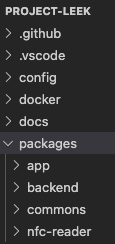
\includegraphics[width=3.8cm]{PackageStruktur.png}
  \caption{Orderstruktur}
  \label{fig:Orderstruktur}
\end{wrapfigure}
Die an das Projekt gesetzten Anforderungen machten die Erstellung mehrerer Applikationen notwendig. Neben einer Benutzeroberfläche, auf der die NFC-Tags
verwaltet werden können, musste die Steuerung des NFC-Readers und ein System zur Speicherung der Daten sowie zum Abspielen der Musik entwickelt werden.
Die dafür benötigten Anwendungen wurden als Microservices konzipiert und umgesetzt. Zur Verringerung des Aufwands der Konfiguration und Wartung wurden die einzelnen Microservices in einem Mono-Repository auf GitHub zusammengefasst.
Jeder Service wurde in einem Unterordner in \textit{packages} angelegt (vgl. Abbildung \ref{fig:Orderstruktur}). Der Ordner \textit{app} enthält die Benutzeroberfläche,
\textit{backend} die Datenbankschnittstelle sowie Logik zur Kommunikation mit dem Musik-Streaming-Anbieter und \textit{nfc-reader} die Applikation zum Steuern und auslesen des am Raspberry Pi angeschlossenen NFC-Readers.
Im Ordner \textit{commons} befinden sich von allen Services gemeinsam genutzte Ressourcen (wie z. B. Modell-Klassen).
Neben den einzelnen Microservices wurden ebenfalls die Dokumentationsdateien wie Setup-Guide, Benutzerdokumentation und Projektbericht im Mono-Repo im Ordner \textit{docs} abgelegt.
Auch die für den Dienst \textit{Docker} benötigten Dateien fanden in dem gleichnamigen Ordner Platz. Die Konfigurationsdateien für \textit{ESLint} und den \textit{Typescript}-Compiler sind im Ordner \textit{config} zu finden.
Auf die Auflistung aller weiteren Dateien wird in diesem Bericht verzichtet. Eine genaue Aufstellung ist dem \textit{GitHub-Repository}\footnote{\url{https://github.com/project-leek/project-leek}} zu entnehmen.
Durch die Zusammenfassung in ein Mono-Repository waren die einzelnen Services für jeden Entwickler jederzeit einfach erreichbar, ohne die Notwendigkeit das Repository zu wechseln.

\subsection{Technologien}
\label{technologien}

\subsubsection{Programmiersprachen}

\paragraph*{TypeScript} $~$ \\
Da alle Teammitglieder bereits Erfahrungen mit JavaScript gesammelt hatten wurde diese zuerst als Programmiersprache vorgeschlagen.
Aufgrund von nicht vorhandener Typisierung wurde sich dann jedoch auf die von Microsoft entwickelte Sprache TypeScript geeinigt. Diese bietet aufgrund des
Aufbaus auf den ECMAScript-6-Standards eine große syntaktische Ähnlichkeit zu JavaScript. Somit fiel das Erlernen der Sprache den Entwicklern relativ leicht.
Durch die starke Typisierung entstehen außerdem weniger Laufzeitfehler, da die entwickelnde Person bereits zur Compile-Zeit auf Typfehler aufmerksam gemacht wird.\cite{Typescript_Typisierung}
Bei der Kompilierung von TypeScript-Code wird dieser zu gültigem JavaScript Code umgewandelt, wodurch auf eine Vielzahl von bereits existierenden JavaScript-Paketen zugegriffen werden konnte.
Außerdem lässt sich Typescript durch Nutzung der Laufzeitumgebung Node.js auch als Backendsprache verwenden und ersparte dem Team damit die Nutzung von verschiedenen Programmiersprachen.


\subsubsection{Frameworks}
Neben der Programmiersprache Typescript setzte das Team verschiedene Frameworks ein, um bei der Entwicklung auf bereits existierenden Lösungen mit weniger Aufwand zu entwickeln.

\paragraph*{Vue.js} $~$ \\
Zur Gestaltung der Benutzeroberfläche für die \textit{leek-box}, die zum Verwalten der NFC-Tags und Steuern der Ausgabegeräte genutzt wird, einigte sich das Team auf die Nutzung des
clientseitigen JavaScript-Webframeworks \textit{Vue.js}\footnote{\raggedright\url{https://vuejs.org/}}
Dieses wurde aufgrund seiner guten Dokumentation und seiner flachen Lernkurve gewählt, wodurch sich der Einstieg für Teammitglieder mit weniger Erfahrung in der Web-Entwicklung leichter gestaltete.
Außerdem bietet das in Vue.js verwendete Entwurfsmuster MVVM (Model View ViewModel) den Vorteil, dass die designaffineren Entwickler sich eher mit dem Frontend beschäftigen können,
während andere am Logik-Code arbeiten. Im Vergleich zu anderen Webframeworks gilt es, laut Benchmarks außerdem als sehr performant.\cite{Vue_Performance}

\paragraph*{Tailwind CSS} $~$ \\
Zur effizienteren Gestaltung der Benutzeroberfläche entschied sich das Team für das Utility-First-Framework \textit{TailwindCSS}\footnote{\raggedright\url{https://tailwindcss.com}}.
Dieses bietet im Vergleich zu anderen CSS-Frameworks wie \textit{Bootstrap} mehr Flexibilität, da statt vorgefertigten Komponenten vielseitig verwendbare Utility-Klassen zur Verfügung gestellt werden,
über die das Design definiert werden kann. So kann das Aussehen von Elementen innerhalb des HTML-Codes festgelegt werden.
Damit steigt die Übersichtlichkeit des Frontend-Codes, da keine separaten CSS-Dateien und -Klassen angelegt werden müssen.
\cite{Tailwind_Vorteile}


\paragraph*{FeathersJS} $~$ \\
Bei der Erstellung des Backends entschied sich das Team zusätzlich das Framework \textit{FeathersJS}\footnote{\raggedright\url{https://feathersjs.com/}} einzusetzten.
Dies ermöglicht komfortable CRUD-Zugriffe\footnote{CRUD = \textbf{C}reate-\textbf{R}ead-\textbf{U}pdate-\textbf{D}elete}  auf verschiedene Services, welche zum Beispiel Datenbanken oder externe APIs sein können.
Durch eine vielzahl von Adapatern können so zum Beispiel Daten in einer Datenbank ohne eigene Implementierung der Schnittstelle verwaltet werden.
Es muss lediglich ein Service erstellt werden, der das generische Interface Service mit Typeparameter der zu verwaltenden Klasse implementiert. (vgl. Abb. \ref{fig:MyService})
\begin{figure}[ht]
  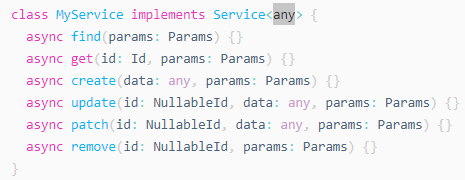
\includegraphics[width=\linewidth]{MyFeathersService.png}
  \setcaptioncitation{https://docs.feathersjs.com/guides/basics/services.html}
  \caption{Implementierung eines ServicesTest}
  \label{fig:MyService}
\end{figure}
Dabei können verschiedenste Protokolle, wie HTTP oder WebSockets zur Datenübertragung verwendet werden.
Das WebSocket-Protokoll bietet hier den großen Vorteil, dass eine persistente Verbindung zwischen Server und Client (Benutzeroberfläche und Backend) besteht.
So können sowohl Client, wie auch Server jederzeit mit der Datenübertragung beginnen, ohne vorher - wie bei HTTP - jedes Mal eine neue Verbindung aufzubauen zu müssen. \cite{WebSockets}
Dadurch kann der Server alle verbundenen Clients bei einem CRUD-Zugriff informieren, sodass alle ohne erneutes Anfragen der Daten den aktuellsten Zustand übermittelt bekommen.
Wird also beispielsweise ein NFC-Tag von Person A geändert, sieht Person B diese Änderung ohne manuelle Aktualisierung der Seite.
Eine weiteres Feature, welches vom Projektteam genutzt wurde ist die integrierte OAuth-Provider-Abstraktionen, die ein einfaches Authentifizieren mit Diensten, wie beispielsweise \textit{Spotify} bei diesem Projekt ermöglicht.
Dies war z.B. nötig, um die den NFC-Tags zugeordnete Musik abspielen zu können.
Darüber hinaus können so auch Nutzerprofile angelegt werden, ohne persönliche Daten, wie z.B. Namen, Email-Adressen und Passwörter, speichern zu müssen.
Nur Authentifizierungstokens des OAuth-Providers werden in der Datenbank hinterlegt.
So konnte ein besserer Datenschutz für die Nutzenden ermöglicht werden.


\subsubsection{Containervirtualisierung (Docker)}
Es wurde lediglich die Anforderung gestellt, dass die Applikation vor allem für mobile Endgeräte optimiert sein soll.
Auf Basis dieser Anforderung evaluierte das Projektteam bekannte Technologien und recherchierte mögliche Alternativen.
Um die Installation der Box möglichst komfortabel zu gestalten, wird auf die freie Containervirtualisierungssoftware \textit{Docker}\footnote{https://www.docker.com/} gesetzt.
Ohne diese Möglichkeit wäre die Installation aufgrund der drei Microservices (Backend, Reverse-Tunnel und NFC-Reader) sehr aufwändig.
Der Vorteil von Docker besteht darin, dass das Team lediglich eine sogenannte \textit{docker-compose} Datei benötigt, in dem die Konfiguration der Docker-Container beschrieben ist.
Es enthält einen Verweis auf die jeweiligen Container-Images, auf denen die Container aufbauen (z. B. leek-backend). Diese Images enthalten bereits alle notwendigen Abhängigkeiten und Programme,
sodass weitere Installationen seitens der Benutzer:innen nicht erforderlich sind.
Außerdem lässt sich das Verhalten der Images durch Umgebungsvariablen weiter konfigurieren. Durch die einfache Auslieferung bietet Docker außerdem den Vorteil der Reproduzierbarkeit.
So können aufgetretene Fehler problemlos von einem Entwickler nachgestellt werden, da Docker das Betriebssystem des Anwenders von der benötigen Umgebung der leek-box abstrahiert.


\subsubsection{Reverse-Tunnel (ngrok)}
Um verschlüsselt vom Frontend (unter \raggedright\url{https://project-leek.github.io} erreichbar) auf das jeweilige Backend einer \textit{leek-box} zuzugreifen, wird der Reverse-Tunnel Dienst \textit{ngrok}\footnote{\raggedright\url{https://ngrok.com/}} verwendet.
Dies ist notwendig, da moderne Browser eine verschlüsselte Verbindung (mit SSL-Zertifikat) zu allen Komponenten auf der Website verlangen, sobald die Website selbst per SSL geladen wird.
Da das Framework jedoch nativ kein HTTPS unterstützt, wird \textit{ngrok} verwendet, um die unverschlüsselten Daten durch einen verschlüsselten Tunnel zum Frontend zu schicken. Damit wird die Anforderung der Verschlüsselten Verbindung erfüllt.
Außerdem soll das Backend unabhängig vom lokalen Netzwerk erreichbar sein, ohne dass eine umständliche Portweiterleitung eingerichtet werden muss. Um dies zu leisten, baut das Backend einen Tunnel zu dem Server mit der bekannten Adresse \url{ngrok.io} auf.
Dabei wird eine zufällige Subdomain im Schema \textit{xyz.ngrok.io} angelegt und dem Benutzer in der Konsole des Backends angezeigt. Diese Adresse kann der Benutzer nun im Frontend (\url{https://project-leek.github.io}) eingeben, um sich mit seiner Box zu verbinden.
\colorbox{red}{Hier Schaubild?}

\subsubsection{Externe Bibliotheken}
\paragraph{Spotify Web API} $~$ \\
\label{SpotifyWebApiNode}
Um die abspielbaren Songs inklusive Cover-Bildern zu ermitteln und diese abzuspielen ist ein Zugriff auf die API eines Musikstreaming-Dienstes notwendig.
Der vom Kunden vorgeschlagene Anbieter war \textit{Spotify}\footnote{\url{https://www.spotify.com}}.
Um den Zugriff auf die Spotify API zu simplifizieren wurde die Bibliothek \textit{Spotify Web API Node}\footnote{\url{https://github.com/thelinmichael/spotify-web-api-node}} verwendet.
Diese bietet bereits die benötigten Methoden, wie z. B. die zum Suchen eines Songs anhand eines Suchbegriffs.
Neben dem Songtitel und der Spotify-Url werden auch die Künstler und die Adresse des Albumcovers mitgeliefert und konnten von den Entwicklern ohne Mehraufwand genutzt werden.
Auch eine Methode zur Ermittlung der verfügbaren Geräte zum Abspielen der Musik stellt die Bibliothek bereit.

\paragraph{NeDB} $~$ \\
Als Datenbank für dieses Projekt wurde die kostenlos verfügbare JavaScript-Datenbank \textit{NeDB}\footnote{\raggedright\url{https://github.com/louischatriot/nedb}} gewählt.
Sie wird verwendet, um die NFC-Tags, Benutzer und den angeschlossenen NFC-Reader zu verwalten.
\textit{NeDB} ist eine auf \textit{MongoDB}\footnote{\raggedright\url{https://www.mongodb.com/}} aufbauende, sehr schnelle JSON Datenbank.
Sie wurde gewählt, da sie eine geringe Komplexität besitzt und weil \textit{FeathersJS} einen Datenbankadapter für diese Datenbank bereitstellt, was den Zugriff auf die Datenbank sowie die Verwaltung der Daten erleichterte.
Außerdem arbeitet die Datenbank inkrementell, was das Risiko auf sehr große Datenbankdateien minimiert.
Diese Eigenschaft war hilfreich, um die Datenbank auf einem Raspberry Pi betreiben zu können.
Zu Beginn des Projekts diskutierte das Team die Technologien, mit denen die \textit{leek-box} umgesetzt werden sollte.
Der Kunde ließ dem Projektteam hierbei sehr viele Freiheiten.

\subsection{Hilfsmittel}
Im Rahmen des Projekts nutze das Team eine Vielzahl von Hilfsmitteln, die die Zusammenarbeit und Produktivität des Teams steigern sollte.
Diese wurden zum einen zu Beginn des Projektes in einer Gruppendiskussion herausgearbeitet oder als Ergebnis der Retrospektiven erprobt.

\subsubsection{Github \& Github IO}
Da alle Teammitglieder, wie auch die Kunden bereits einen Account bei dem Dienst \textit{GitHub} besaßen, wurde die Entscheidung getroffen, diesen als Hoster für \textit{Git-Remote-Repositories} einzusetzen.
Aufgrund der bereits gewonnenen Erfahrung mit diesem Dienst und der Fokussierung auf quelloffene Software, stellte er für dieses Projekt die ideale Umgebung zur Quellcodeverwaltung und Kollaboration dar.

\paragraph{Kollaboration} $~$ \\
Mit dem Anspruch das Produkt auch nach Projektende fortzuführen, wurden auch die Projektmanagement Funktionen von GitHub verwendet. Die einzelnen Aufgaben bzw. Arbeitspakete (\textit{Issues}\footnote{Da das Team größtensteils den Begriff \textit{Issue} nutzte, wird dieser auch fortlaufend hauptsächlich verwendet.}) wurden in einem \textit{Issue Board} den verschiedenen Arbeitsstatus\footnote{Status = Backlog, Todo, In Progess, Review und Done}
zugeordnet. Außerdem konnten verschiedene Informationen, wie z. B. der Sprint bzw. \textit{Milestone\footnote{Auch hier wird im weiteren Verlauf eher der Begriff Milestone oder Meilenstein verwendet.}} in dem das Ticket abgeschlossen sein soll oder der bearbeitende Entwickler dokumentiert werden.
Da diese Ansicht ebenfalls nach diversen Eigenschaften gefiltert werden kann, konnte sich jeder Entwickler schnell einen Überblick über den aktuellen Projektstand verschaffen.
Das Team setzte zur Unterstützung außerdem den \textit{Renovate-Bot}\footnote{\raggedright\url{https://github.com/renovatebot/renovate}} ein, welcher die Tickets automatisch anhand von verschiedenseten Events verschob und einen Branch anlegt, wenn sich ein Entwickler einem Ticket zuordnet.
\\~\\
Eine weitere Funktionalität von GitHub, die in diesem Projekt genutzt wurden sind die sogenannten \textit{Actions}\footnote{\raggedright\url{https://github.com/features/actions}}.
Sie ermöglichen automatisierte Tests, die den Quellcode und die Anwendung als Gesamtkonstrukt auf verschiedenste Fehler prüfen und frei konfigurierbar sind.
In diesem Projekt wurden die folgenden vier Tests durchgeführt um die Änderungen vor der Übertragung in den Master-Branch zu validieren:
\begin{enumerate}
  \item \textbf{build}: Wird die Software fehlerfrei gebaut?
  \item \textbf{lint}\footnote{Tool zur statischen Codeanalyse}: Ist der Quellcode in gutem Stil geschrieben?
  \item \textbf{test}: Sind die geschrieben Unit-Tests erfolgreich?
  \item \textbf{typecheck}: Sind alle Typen kompatibel?
\end{enumerate}
Sind alle Tests erfolgreich, ist die Änderung technisch nutzbar.
\\~\\
Außerdem wurde die in GitHub existierende Funktionalität der Pull Requests verwendet. Beim \textit{Pushen}\footnote{Hochladen der Änderung vom Entwickler-PC auf das Repositoty auf GitHub}
werden die Änderungen automatisch in dem den Branch betreffenden Pull Request angezeigt (wenn vorhanden).
Jeder Pull Request enthält allgemeine Informationen, welchem Zweck er dient und von wem die Änderung durchgeführt wird. Außerdem wird das Ergebnis der automatisierten Tests (\textit{GitHub Actions}) angezeigt.
Das Projekt ist so konfiguriert, dass die Übernahme der Änderung des Pull Requests nur möglich ist, wenn mindestens zwei andere Entwickler diesen Änderungen
durch Code Reviews zugestimmt haben und alle automatisierten Test erfolgreich abgeschlossen wurden. Ist dies der Fall, kann die Änderung in den Master-Stand übertragen werden.
Für die Code-Reviews wurde ebenfalls die GitHub interne Funktionalität genutzt, die bequeme Änderungsvorschläge ermöglicht.

\paragraph{Github Pages} $~$ \\
Zum Bereitstellen des Frontends der \textit{leek-boxen} wird der Dienst GitHub Pages verwendet. Dieser stellt pro Organisation und Repository eine kostenlose URL xyz.github.io zur Verfügung.
Dabei werden unter dieser statische Dateien, wie zum Beispiel die einer Website: \textit{.html}, \textit{.css}, \textit{.js}, aus einem bestimmten Branch oder einem Ordner bereitgestellt.
Die Konigurationsanforderungen für ein einfaches Website-Hosting sind somit minimal.

\subsubsection{Visual Studio Code \& WSL}
Als Entwicklungsumgebung in diesem Projekt wurde \textit{Visual Studio Code} verwendet. VSCode war allen Gruppenmitgliedern bereits bekannt und wurde von vielen auch regelmäßig verwendet.
Die IDE beherrscht den Umgang mit allen für das Projekt benötigten Dateitypen und ist durch eine Vielzahl an kostenlos angebotenen Erweiterungen (Extentions) sehr anpassbar an die Projektbedürfnisse.
So wurden in diesem Fall unter anderem die Erweiterungen \textit{Vetur} (für Vue.js), \textit{LaTeX Workshop}  (für die Erstellung dieses Berichts) und \textit{Tailwind CSS IntelliSense} (Für Auto-Vervollständigung der CSS Klassen von Tailwind) verwendet.
Außerdem bietet \textit{Visual Studio Code} eine komfortable Anbindung\footnote{\raggedright\url{https://code.visualstudio.com/docs/remote/wsl}} an das
\textit{Windows Subsystem für Linux (WSL)}\footnote{\raggedright\url{https://docs.microsoft.com/de-de/windows/wsl/about}}, welches eingesetzt wurde, um eine möglichst homogene Arbeitsumgebung innerhalb des Teams sicherzustellen
und neben der gleichen IDE auch auf Betriebssystemen der gleichen Kernel-Infrastrukur (UNIX) zu arbeiten. Dies erleichterte insbesondere die Arbeit mit \textit{Docker} deutlich.

\subsubsection{Prototyping (Figma)}
\label{figma}
Zur Abstimmung auf ein Design für die Benutzeroberfläche wurden vor der Entwicklung Prototypen der benötigten Komponenten mittels des webbasierten
Prototyping-Tools \textit{figma}\footnote{https://www.figma.com/} konzipiert. So konnten neben dem Design auch Abläufe in Form von \glqq Click-Dummys\grqq{} erstellt werden und mit dem Kunden abgestimmt werden.
\textit{Figma} wurde verwendet, da es einen kollaborativen Zugriff ermöglicht, kostenlos ist und bereits Erfahrung mit der Plattform bestand

\subsubsection{Lucidchart}
\label{Lucidchart}
Um Abläufe schon vor dem Prototyping skizziert darstellen zu können wurde außerdem die webbasierte Plattform \textit{Lucidchart}\footnote{\raggedright\url{https://www.lucidchart.com/}} verwendet.
Hier wurde neben der initial erstellten Produktübersicht auch mehrere Aktivitätsdiagramme erstellt, die aus vom Projektteam entwickelten und mit dem Kunden abgestimmten User-Stories entstanden sind.
Diese sind im Anhang unter \colorbox{yellow}{Verweis einfügen!} zu finden.
Auch diese Plattform ermöglicht den gleichzeitigen Zugriff und war den Entwicklern bereits bekannt, was die Notwendigkeit der Einarbeitung eliminierte.
\subsection{Entwicklungszyklus}
Während der Umsetzung der \textit{leek-box} durchlief jedes Teammitglied für jedes \textit{Issue} den am Anfang des Projekts festgelegten und
durch die Retrospektiven optimierten Zyklus.
\\~
Am Anfag steht die Auswahl eines \textit{Issues} aus der Spalte \textit{ToDo} des \textit{Issue Boards}.
Nach Identifikation weist sich der Entwickelnde dem Ticket zu. Daraufhin erstellt der verwendete Bot automatisch einen \textit{Branch}
in dem Schema \textit{[Ticketnummer]-[Ticketname]}. Nun kann mit der Arbeit in \textit{Visual Studio Code} begonnen werden.
\\~
Die Änderungen sollten möglichst kleinschrittig aber sinnvoll \textit{comittet} und anschließend \textit{gepusht} werden.
GitHub erkennt automatisch die neuen \textit{commits} und erfragt, ob ein neuer \textit{Pull-Request} angelegt werden soll.
Dieser hat initial den Status \textit{Open}.
Wenn die Aufgaben des \textit{Issues} noch nicht abgeschlossen sind, wird der Status auf \textit{Draft} gesetzt.
\\~
Nach dem \textit{push} aller Änderungen, wird das Ergebnis der automatisierten Tests (\textit{GitHub Actions}) ermittelt. Treten hierbei Fehler auf,
werden diese geprüft und behoben. Sind alle Tests erfolgreich, betätigt der Entwickelnde die Schaltfläche \textit{Ready for Review}.
Wenn ein:e Entwickler:in, diesen \textit{Pull-Request} sieht, wird ein \textit{Code-Review} durchgeführt.
Hierzu wird der Branch in die IDE geladen und die Funktionalität verifiziert. Anschließend wird die Code-Qualität geprüft.
Dafür werden die geänderten Dateien im Pull-Request betrachtet. Anmerkungen können in Form
von Kommentaren an einzelne oder mehrere Zeilen angefügt werden. Bei Änderungsvorschlägen können diese über eine \textit{suggestion}
getätigt werden. Ist der komplette Code geprüft wird entschieden,
ob die Änderungen angenommen (\textit{approve}) werden oder eine Änderungsanforderung gestellt wird (\textit{Request changes}).
\\~
Im Falle von Änderungsanforderungen werden diese umgesetzt und ein erneutes Review angefordert. Dies geschiet zyklisch, bis die Änderungen angenommen werden.
Sind die Änderungen durch zwei \textit{Code-Reivews} bestätigt worden, werden sie mit der Schaltfläche \textit{Mege into master} übertragen.

\subsection{Testing}
Das Team entschied sich zu Beginn der Produkt-Entwicklung dafür, Tests zur Verbesserung der Codequalität durchzuführen.
Quellcode Tests lassen sich in statische und dynamische Tests unterteilen.

\subsubsection*{Statische Tests}
Im Allgemeinen untersuchen statische Tests nur Textdokumente und betrachten im Gegensatz zu dynamischen Tests nicht das Verhalten zur Laufzeit.
Dies ermöglicht eine häufige und kontinuierliche Nutzung von Tests dieser Art.
Zwei der prominenten Varianten statischer Tests, Linting und Reviews, wurden in diesem Projekt genutzt.

\paragraph*{Linting}$~$ \\
Beim Linting wurde der Code auf syntaktische Korrektheit geprüft.
Auch manche semantische (laufzeitunabhängige) Aspekte wurden untersucht.
So konnten kleinere Denkfehler und Flüchtigkeitsfehler, wie z. B. fehlende Kommata, schnell gefunden und behoben werden.
Hierfür wurde das Analyse-Werkzeug \textit{ESLint}\footnote{\raggedright\url{https://eslint.org/}} genutzt.
Für diese Werkzeug war zusätzlich auch eine Erweiterung\footnote{\raggedright\url{https://marketplace.visualstudio.com/items?itemName=dbaeumer.vscode-eslint}} für die Entwicklungsumgebung verfügbar.
Mit dieser konnten die Ergebnisse des Linting direkt im Code angezeigt werden.
Dies machte den Arbeitsprozess wesentlich zeiteffizienter.
Zusätzlich wurde auch die Erweiterung \textit{Vetur}\footnote{\raggedright\url{https://vuejs.github.io/vetur/}} genutzt.
Diese stellte die selben Funktionalitäten für den Vue-Framework spezifischen Code zur Verfügung.
\\
Darüber hinaus boten diese Erweiterungen auch Formatierungshilfen mit übertragbaren Konfigurationen.
Durch deren Nutzung konnte ein konsistenter Code-Stil innerhalb des Teams ermöglicht werden.
Dies legte den Grundstein für lesbaren Code und ermöglichte successive effizientes Arbeiten.

\paragraph*{Reviews}$~$ \\
Teil des Deployment Cycles waren auch Reviews der aktive Änderungen.
Bei diesen wurde der neue bzw. geänderte Quellcode von mindestens zwei anderen Teammitgliedern überprüft.
Untersucht wurden vor allem semantische Fehler, Lesbarkeit, Wartbarkeit und Vollständigkeit.
Hierfür gab es keinen formalen Plan, allerdings war die Review-Oberfläche von GitHub sehr hilfreich.
In dieser wurde eine Änderungsansicht (\textit{diff}) des zu überprüfenden Codes angezeigt.
So waren alle Teile des neuen Codes auf einen Blick einsehbar.
Darüber hinaus bot die Review-Oberfläche auch die Möglichkeit direkt im Code einzelne oder mehrere Zeilen zu kommentieren.
So konnten auch Änderungsvorschläge gemacht und direkt übernommen werden.
Dies sorgte für einen effizienten Review-Prozess.

\subsubsection*{Dynamische Tests}
Als dynamische Tests wurden in diesem Projekt Anwendungsfall-basierte Tests genutzt.
Bei dieser Art von Test werden auf User-Stories aufbauende Testfälle herangezogen.
Diese Testfälle werden Schritt für Schritt \glqq durchgespielt\grqq.
Dabei wird überprüft, ob das tatsächliche Ergebnis dem erwartetem entspricht.
Die meisten Test  dieser Art wurden als Integrations-Tests durchgeführt.
Bei diesen wurde die Änderungen im Kontext der bestehenden Software getestet.
So konnte vor allem das Zusammenspiel von Frontend und NFC-reader mit dem Backend gut überprüft werden.
Aufgrund der Komplexität dieser Kontrollen wurden diese manuell durchgeführt und nicht automatisiert.
Diese Tests waren Teil des Deployment Cycles und wurden so in den meisten Fällen parallel zu den Reviews durchgeführt.
\\~\\
Ein gewisser Teil der anwendungsfallbasierten Test fand auf der Ebene von Code-Funktionen (\textit{Units}) statt.
Diese Unit-Tests wurden zur einfacheren Wiederholbarkeit automatisiert.
Dazu wurde das JavaScript-Test-Framework \textit{Jest}\footnote{\raggedright\url{https://jestjs.io/}} genutzt.
Dieses wurde gewählt, da sich Tests hiermit sehr intuitiv und ohne großen Lernaufwand schreiben ließen.
Auch diese Tests waren Teil des Deployment Cycles und wurden so bei jedem Pull-Request automatisch ausgeführt.


\subsection{Projekt Meilensteine}

\subsubsection*{Meilenstein 1}
Die Laufzeit des ersten Meilensteins erstreckte sich vom 29.10.2020 bis zum 11.11.2020 und war auf die Planung, Struktur und das Vorgehen des Projektes fokusiert.
%Ziel
Zum Ende des Meilensteins sollte die Struktur und das Grundgerüst für das Projekt fertiggestellt sein.
Hierfür sollte das Konzept der Software-Architektur sowie die genutzten Technologien (später Technologie-Stack genannt) auf Basis einer Anforderungsanalyse mit dem Kunden festgelegt werden.
Außerdem sollten die ersten Tickets in das Backlog eingetragen werden.
Auch musste das Projekt dahingehend geplant werden, dass jedem Teammitglied durchgehend zu bearbeitende Arbeitspakete zur Verfügung standen.
Um ein schnellen und reibungslosen Start für die Entwicklung zu gewährleisten, sollte das Repository entsprechend vorbereitet werden.
%Probleme
Das Team musste das Projekt so entsprechend planen, dass jedes Teammitglied durchgehend sinnvoll arbeiten konnte.
%Lösungen
Durch bereits vorhandene Erfahrung mit verschiedenen Technologie-Stacks und ähnlichen Problemen, wurde sich auf den Technologie-Stack geeinigt
Die verwendeten Technologien sind dem Abschnitt \ref{technologien} zu entnehmen.
Um für jedes Teammitglieds ein sinnvolles kontinuierliches Arbeiten zu gewährleisten, einigte sich das Team auf einen ständig gefüllten Ticket-Pool im Repository, sodass jederzeit selbstständig eine Aufgabe gefunden und bearbeitet werden konnte.
%Product Increment
Das Ergebnis des ersten Meilensteins bestand, abweichend von den späteren, nicht in einem Produkt Inkrement, sondern legte die Grundbausteine für die Entwicklung und das Teamwork.
Neben dem bereits erwähnten Technologie-Stack, wurde als Host für die Applikation ein Raspberry Pi gewählt.
Für die Entwicklung wurde ein Mono-Repository mit \textit{lerna}\footnote{https://lerna.js.org/} aufgesetzt, welches Front- und Backend zusammenfasste.
Durch die Anforderung der Veröffentlichung als Open Source Projekt wurde eine verständliche und hilfreiche Dokumentation nötig, die einem Benutzer die Installation und Verwendung der \textit{leek-box} aufzeigt.
So wurde dem Repository eine einleitende Readme und ein \glqq How to Contribute\grqq{} Guide hinzugefügt.
%Retrospektive
Nach dem ersten Meilenstein fand noch keine nennenswerte Retrospektive statt.

\subsubsection*{Meilenstein 2}
Der zweite Meilenstein wurde für den Zeitraum vom 11.11.2020 bis zum 25.11.2020 angesetzt.
Ziel war es, die ersten Grundbausteine für das Projekt legen. Damit das Team ein generelles Verständnis des Technologie-Stacks entwickeln konnte,
sollte jedes Teammitglied eine \glqq Hello-World\grqq{} Übungsaufgabe absolvieren. Diese beinhaltete das Anlegen eines Feathers-Services für ein virtuelles
Haustier im Backend und die Darstellung im Frontend. Auch die Grundstruktur für den Bericht zu dem Projekt sollte in diesem Milestone erstellt werden,
um den Fortschritt, Probleme und Erkentnisse zeitnah dokumentieren zu können.
\\~\\
\paragraph*{Hello-World (Pet)} $~$ \\
\label{HelloWorld}
Zur Umsetzung setzten sich die Entwickler mit der Dokumentation von Feathers auseinander um einen
Überblick über die notwendigen Klassen und Konstrukte zu erhalten. Zuerst musste eine Klasse erstellt werden, in der der Aufbau des Haustierts modeliert
wurde. Sie beinhaltete Attribute wie \glqq Name\grqq{} oder \glqq Id\grqq. Auf dieser Basis wurde anschließend ein Feathers-Service in Form einer
Klasse erstellt. Diese implementierte das von \textit{Feathers} bereitgestellte generische Interface \textit{Service<T>}. Als Typparameter wurde hier
die zuvor erstellte Model-Klasse angegeben. Um z. B. Objekte der Klasse \textit{NicksPet} zu verwalten wurde folgender Service angelegt:
\begin{lstlisting}
  class NicksPetService implements MyService<NicksPet> {
    id! : number;
    name! : string;

    constructor(_id: number, _name: string) {
      this.id = _id;
      this.name = _name;
    }
  }
\end{lstlisting}
In dieser Klasse war außerdem ein Verweis auf eine weitere erstellte Klasse (Model) aufgeführt, welche bestimmt, mit welcher Schnittstelle oder API die Daten
verwaltet werden sollen (in diesem Fall mit der durch \textit{Feathers} bereitgestellten Schnittstelle für die Datenbank \textit{NeDB}).
Mit dem Erstellen dieser drei Klassen (NicksPet.class.ts, NicksPetService.ts und NicksPet.model.ts) waren die benötigten Komponenten zur Verwaltung vorhanden und
und die Arbeit im Backend abgeschlossen. Der nächste Schritt beinhaltete die Implementierung der Steuerelemente zum Verwalten der Daten im Frontend.
Aufgrund der erhöhten Komplexität der Einarbeitung in mehrere teilweise komplett unbekannte Frameworks zur selben Zeit, bestanden bei dieser Aufgabe
einige Startschwierigkeiten, welche allerdings durch die große Hilfsbereitschaft der erfahreneren Teammitglieder überwunden werden konnte.
\\~\\
Im Frontend wurde pro Haustier je ein \textit{component} zur Anzeige eines Haustiers angelegt,
welches zusammen mit den Steuerelementen zum Anlegen, Löschen und Bearbeiten in einer \textit{View} platziert wurde.
Aufgrund der je nach Entwickler sehr unterschiedlichen Implementierung der \textit{component} wird hier auf eine ausführliche Beschreibung verzichtet.

\paragraph*{NFC-Tags auslesen} $~$ \\
\colorbox{red}{Hier bei Bedarf noch weiter ausführen}
Neben der Umsetzung des Hello-Worlds sollte sich mit dem Raspberry Pi und dem NFC-Reader auseinandergesetzt und das Auslesen der NFC-Tags implementiert werden. Diese Anforderung geriet mangels ausreichender Notizen beim ersten Review vorerst
in Vergessenheit, sodass sich das Team einige Tage vor Sprintende nicht sicher war, ob diese Anforderung bis zum Review umgesetzt werden könnte.
Um das Sprintziel nicht zu gefährden, mussten gegen Ende des Sprints Überstunden geleistet und das Feature konnte ins Produktinkrement aufgenommen konnte.
\\
Zur Umsetzung wurde im Backend die Klassen und der Service zur Verwaltung eines NFC-Readers und NFC-Tags
analog zu dem in \ref{HelloWorld} beschriebenen Vorgehen erstellt.
Außerdem wurde der Microservice \textit{nfc-reader} in der Projektstruktur unter \textit{packages}
angelegt. Dieser nutzt die Bibliothek \textit{Evdev}\footnote{https://github.com/PixnBits/node-evdev}, welches ein Interface für die Events der angeschlossenen
Eingabegeräte vom Linux-Kernel, wie in unserem Fall den NFC-Reader, bereitstellt. Dies ist möglich, da der NFC-Reader sich wie eine Tastatur verhält. Er
simuliert dabei eine Tastatureingabe mit dem Text der NFC-Tag-ID. Zur Nutzung wurden zwei Klassen erstellt. Zum einen die NFC-Reader Klasse
(im NFC-Reader Package), welche jeden simulierten Tastendruck des NFC-Readers abfängt, bis ein Zeilenumbruch (0A HEX) empfangen
wird und anschließend ein Event auslöst, welches die eingescannte ID beinhaltet. Die Hauptklasse nimmt dieses Event entgegen (Event-Listener) und setzt mittels des
NFC-Reader Services den aktuell anliegenden Tags (\textit{currentTag}) auf die übergebene ID. Durch die Nutzung von \textit{Web-Sockets} und \textit{Vue.js}
kann diese Änderung sofort im Frontend angezeigt werden. Aufgrund der potentiell hohen Komplexität des Abspielens von Musik wurde diese Funktionalität für den
folgenden Milestone eingeplant und vorerst lediglich die Anzeige der NFC-ID als JSON-String umgesetzt.
\\
\colorbox{red}{Hier bei Bedarf noch weiter ausführen, aber wäre sehr ins Detail gegeangen}
Für den Microservice wurde anschließend ein Docker-Image kreiert, welches eine einfache und gleichzeitig optionale Auslieferung zur restlichen Installation
ermöglicht. Dies bringt den Vorteil, dass auch auf einem anderen System (wie z. B. einem esp32) integrierte NFC-Reader, statt des aktuellen genutzt werden können.

\paragraph*{Prototyping der Beutzeroberfläche} $~$ \\
Damit die Entwicklung zeitnah starten konnte, wurden die ersten Mockups für die Benutzeroberfläche erstellt.
Mithilfe des Prototyping-Tools \textit{figma} (vgl. \ref*{figma}) wurden Prototypen für die Start- , die Hauptansicht und die Ansichten
für das Bearbeiten und Anlegen von NFC-Tags erstellt (Eine Übersicht über das erstellte Design ist im Anhang unter \ref*{FigmaDesigns} zu finden).
Nach dem Design wurden die Ansichten in \textit{Click-Dummys} umgewandelt, um dem Kunden im folgenden Review einen Überblick über das Verhalten der
Benutzeroberfläche zu verschaffen.

\paragraph*{Review} $~$ \\
Dank des großen Engagements und der Bereitschaft Überstunden zu leisten, konnte dem Kunden zum Review ein neues Produktinkrement übergeben werden.
Das Produkt wurde um ein erstes User Interface erweitert, welches die Tag-ID vom angelegten NFC-Tags anzeigen konnte.
Der NFC-Reader wurde mit dem Raspberri Pi verbunden und als ein auslieferbares Docker Image bereitgestellt.
Auch wurden für die Entwicklung automatisierte Tests erstellt, welche neuen Code auf etablierte Code-Konventionen und Lauffähigkeit überprüften.

\paragraph*{Retrospektive} $~$ \\
Vor allem der Einsatz und das Know-How vom Teammitglied Anton wurde hier wertgeschätzt, welcher sich um die Automatisierung von Tests und Deployment kümmerte.
Auch das Gruppenklima wurde sehr gelobt und angemerkt, dass die Zusammenarbeit, Kommunikation und die regelmäßigen Meetings sehr positiv wahrgenommmen wurden.
Das Team konnte bei der Umsetzung dieses Meilensteins viel über die Funktionsweise der Frameworks \textit{Feathers}, \textit{Vue.js} und \textit{Tailwind} lernen.
Darüber hinaus kamen viele das erste mal Automatisierungsprozessen, Code-Reviews und Pull Request in Kontakt.
Das Team bemängelte bei dem Meilenstein aber auch, dass der Kundenwunsch zu spät behandelt wurde und die Prioritäten falsch gesetzt wurden.
Somit wurde als Verbesserungen für die nächsten Meilensteine eine bessere Koordination und Aufgabenverteilung vorgeschlagen.

\subsubsection*{Meilenstein 3} $~$ \\
Vom 25.11.2020 bis zum 17.12.2020 fand die Umsetzung von Meilenstein drei statt.

\paragraph*{Mockup Überarbeitung} $~$ \\
Die erstellten Mockups für die Benutzeroberfläche sollten in diesem Sprint basierend auf dem Feedback von macio finalisiert werden.
Das Ergebnis führte bei den Entwicklern anfänglich zu etwas Unsicherheit, da das Team nur aus Studierenden des Studiengangs
Informationstechnologie bestand, welche mit dem Thema Usability, abgesehen von dem Modul
\textit{Usability Engineering}\footnote{\raggedright\url{https://moduldatenbank.fh-kiel.de/de-DE/Module/Details/0de99d45-efc9-437a-a190-24d539b2a1d8}}
wenig Kontakt und haben und darüber hinaus wenig persönlichen Erfahrungen in dem Themenbereich gesammelt hatten.
Diese Schwierigkeiten wurden durch offene Kommunikation an macio weitergegeben, die zur Problemlösung einen ihrer Designer baten,
bei der Entwicklung des Designs zu unterstützen.

\paragraph*{Flow-Charts} $~$ \\
\begin{wrapfigure}{r}{0cm}
  %\vspace{-30pt}
  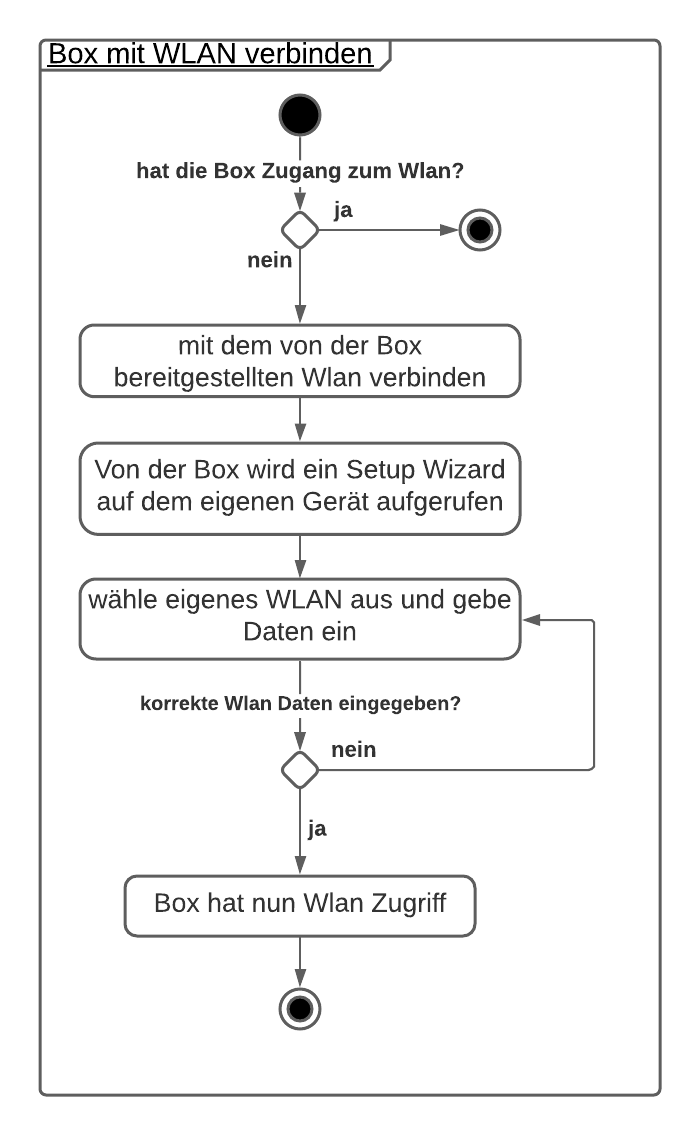
\includegraphics[width=0.45\textwidth]{ConnectToWIFI.png}
  \caption{Flowchart: Connect to WIFI}
  \label{fig:ConnectToWifi}
\end{wrapfigure}
Außerdem wurden die im letzten Sprint erstellten \textit{User Stories} als Grundlage für die Entwicklung von \textit{Flow-Charts} verwendet.
Diese wurden mit dem Online-Tool \textit{Lucidchart} (vgl. \ref*{Lucidchart}) erstellt und sind im Anhang unter \ref*{FlowCharts} zu finden.
Sie erleichterten die Umsetzung der Deisgn-Mockups, indem sie notwendigen Abläufe visualisierten.
Dank dieses Zwischenschrittes konnten auch die nicht durch Mockups visualisierte Funktionen, wie das Verbinden der Box mit dem WLAN, zuerst logisch skizziert
werden, bevor sie programmiert wurden. Dadurch konnte innerhalb des Teams auführlich die beste Methode diskutiert werden, um die bestmögliche Usability
für den Benutzer sicherzustellen. Außerdem konnten sie auch dem Kunden vorgelegt werden, um etwailige Miskommunikation bei der Anforderungsanalyse zu vermeiden
und so die Wahrscheinlichkeit auf spätere Änderungen wichtiger Funktion zu senken. Die Erstellung dieser \textit{Flow-Charts} hat mit übereinstimmender
Meinung aller Teammitlgieder die spätere Programmierung maßgeblich effizienter gestaltet und wurde auch vom Kunden sehr geschätzt.


\paragraph*{Musik abspielen} $~$ \\
Auch der vom Kunden geäußerte Wunsch, beim Einlesen eines NFC-Tags die entsprechende hinterlegte Musik abzuspielen, sollte in diesem Milestone umgesetzt werden.
Dafür setzte sich ein Teil des Teams intensiv mit der \textit{Spotify-API}\footnote{https://developer.spotify.com/documentation/web-api/} auseinander.
Hierbei entdeckten die Entwickler die Biblothek \textit{Spotify Web API node} (vgl. \ref*{SpotifyWebApiNode}), welche den Zugriff auf die \textit{Spotify-API},
abstrahiert und so den Zugriff auf diese erleichtert. Die Bibliothek wurde in Kombination mit \textit{Feathers-Hooks}
\footnote{https://docs.feathersjs.com/api/hooks.html} verwendet. Hooks sind Funktionen, die z. B. vor oder nach einem Feathers Service Aufruf ausgeführt werden
können. In diesem Fall beinhaltet der angelegte \textit{playSpotify} Hook einen Aufruf der Methode \textit{play} der \textit{Spotify Web API Node}, die den Song
hinter der \textit{URL} des mitgegebenen NFC-Tags abspielt. Dieser Hook ist an die \textit{patch} Methode es NFC-Reader Services angehängt, sodass dieser im
Anschluss an die \textit{patch} Methode, die den Eintrag des \textit{attachedTag} des NFC-Readers aktualisiert, aufgerufen wird.

\paragraph*{NFC-Tags scannen emulieren} $~$ \\
Da während des Projekts nicht alle Entwicker kontunierlichen Zugang zu einem NFC-Reader hatten wurde im Zuge dieses Milestones außerdem die Möglichkeit
geschaffen, das Scannen eines NFC-Tags zu emulieren. Hierfür wurde ein \textit{Shell-Script} erstellt, welches einen \textit{HTTP PATCH request} an
das Backend schickt. Dadurch wird der \textit{attachedTag} des NFC-Readers auf Basis eines übergebenen Parameters gesetzt. So kann zum Beispiel ein NFC-Tag mit
der ID 12345 emuliert werden, indem im Terminal der Aufruf \textit{./simulate-read.sh 12345} durchgeführt wird, ohne dass der Entwickler einen physischen NFC-Reader
an seiner Entwicklungsmaschine angeschlossen haben muss. So konnten Funktionen wie das Anlegen eines neuen NFC-Tags von jedem Entwickler durchgeführt werden.


\paragraph*{Entwicklung des Welcome Screens mit Authentifizierung} $~$ \\
\begin{wrapfigure}{r}{5cm}
  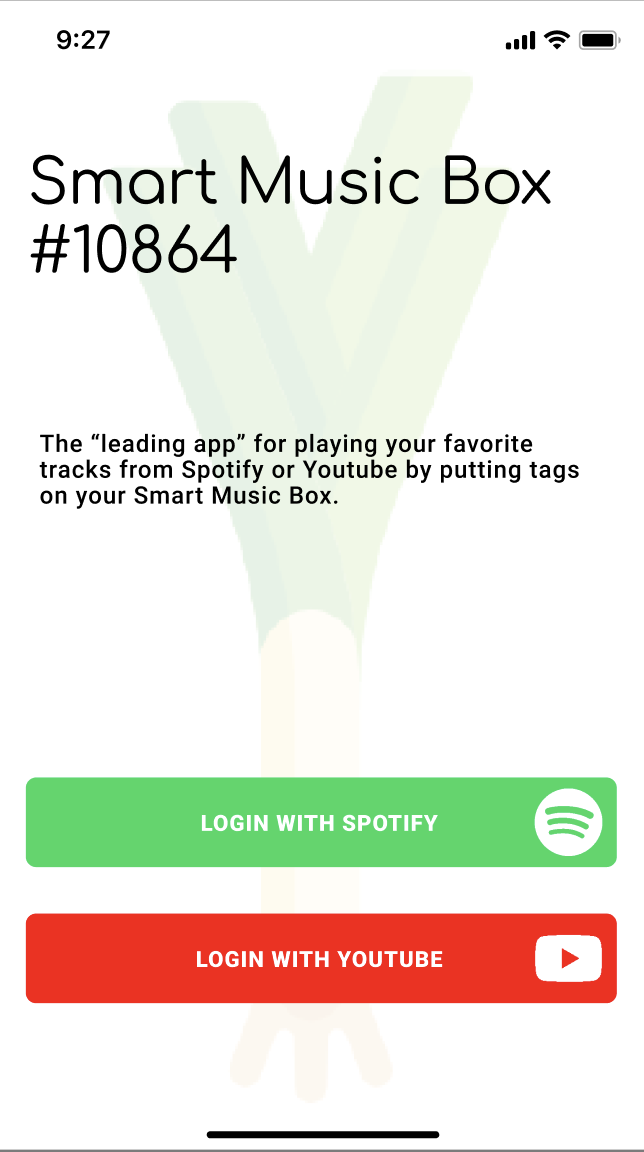
\includegraphics[width=4.8cm]{WelcomeScreenV1.png}
  \caption{Orderstruktur}
  \label{fig:Welcome Screen (Version 1)}
\end{wrapfigure}
Um das in diesem Milsteone erstellte Feature des Abspielens von Musik sinnvoll nutzen zu können, musste sich auch mit der Authentifizierung mit Spotify beschäftigt
werden. Dafür wurde das offene Protokoll \textit{OAuth} verwendet, welches bereits in \textit{Feathers} abstrahiert implementiert ist. Zur Nutzung dieses
Protokolles wurde eine sogenannte \textit{Stragegy} angelegt, welche den für die Anmeldung notwenigen Datenaustausch mit Spotify ermöglicht.
Die dafür nötige \textit{Stragegy} mit dem Namen \textit{SpotifyStrategy} wird durch eine Klasse realisiert, welche von der Feathers bereitgestellten Klasse
\textit{OAuthStragegie} erbt. Bei der Anmeldung eines Benutzer wird von Spotify ein JWT-Token an das Backend übergeben. Ein JWT-Token besteht aus einem Base64
enkodiertem Text, welcher beliebige Daten beinhalten kann. Diese Daten sind unverschlüsselt (nur enkodiert) in dem Token hinterlegt und werden
durch eine Signatur auf ihre Integrität überprüft. Der von Spotify übermittelte JWT-Token enthält in diesem Fall die ID, E-Mail und den Namen des
Benutzers. Diese Daten werden extrahiert und sofern der Benutzer nicht bereits in der Datenbank vorhanden ist, zum Anlegen eines neuen Benutzers verwendet.
Sollte der Benutzer jedoch bereits in der Datenbank existieren, so wird dieser gegebenenfalls aktualisiert. Da sich jeder Benutzer vor der Verwendung der App
zuerst  mit einem gültigen Token identifizieren muss, wird bei möglichen Änderungen der Stammdaten in Spotify sofort immer der Datenbankeintrag in Feathers
aktuell gehalten.
\\~\\
Zum Beginn der Umsetzung wurde auf Basis des Mockups ein View in der Benutzeroberfläche (\textit{app} package) erstellt. Dieser enthält als Steuerelemente Infos
über den Namen des Produkts - \textit{leek-box} - und einen kurzen Untertitel, sowie einen \glqq Anmelden mit Spotify\grqq{} Button, der den OAuth-Prozess startet.
Diese Seite wurde mittels des \textit{Vue Routers} so konfiguriert, dass sie nur aufgerufen wird, wenn der Benutzer nicht angemeldet, also kein JWT-Token
vorhanden ist. Ist ein JWT-Token vorhanden, wird der Nutzer bei dem versuchten Aufruf dieser Seite automatisch auf die Hauptseite weitergeleitet.

\paragraph*{Veröffentlichung der App auf Github Pages} $~$ \\
Zur Veröffentlichung unseres Frontends der \textit{leek-box} verwenden wir den Dienst Github Pages welcher ein Webhosting von statischen Dateien unter einer xyz.github.io URL anbietet.
Das Team verwendete für das Frontend ein separates Repository \textit{project-leek/project-leek.github.io} mit der URL project-leek.github.io.
Nach dem Continous-Delivery Verfahren, baut die Pipeline des eigentlichen project-leek Repositories automatisch nach jedem Merge auf den master Branch das \textit{app-package}.
Dafür wird das Build-Tool des \textit{app-package}s aufgerufen und die dabei enstanden statischen Dateien werden von dem Pipeline Plugin
\textit{github-pages-deploy-action}\footnote{\raggedright\url{https://github.com/JamesIves/github-pages-deploy-action}} aus der Pipeline in das separate
\textit{project-leek/project-leek.github.io} Repository für den GitHub Pages Dienst kopiert. Somit befindet sich unter project-leek.github.io immer die aktuellste Version der App.
Dies hat den Vorteil, dass Änderungen wie zum Beispiel Bugfixes und neue Features dem Endanwender schnellst möglich zur Verfügung gestellt werden können ohne das auf einen Release-Plan Rücksicht genommen werden muss.

\paragraph*{Review \& Retrospektive} $~$ \\
Zusätzlich zu dem Wunsch, beim Anlegen eines NFC-Tags die jeweilig hinterlegte Musik abzuspielen, war zum Review auch das Einloggen
in einen bestehenden Spotify Account möglich. Jegliche Neuerung auf dem Master wurden außerdem auch auf Github.io veröffentlicht, sodass der Kunde jederzeit
den Fortschritt ermitteln konnte.
\\
Die vom Team durchgeführte Retrospektive ergab, dass die Problembewältigung durch die Anwendung von Pair Programming in diesem Sprint optimiert werden konnte.
Auch der Workflow mit Github und den Pull Request wurde verinnerlicht sowie Code Reviews verstärkt durchgeführt. Das Team lernte in diesem Sprint
Vue Hooks und die Stärken von Feathers in Verbindung mit OAuth kennen. Festgestellt wurde außerdem, dass einige Tickets weiterhin stark voneinander abhängig waren,
weshalb das Bearbeiten einiger Aufgaben nicht direkt möglich war. Da Abhängigkeiten teilweise unvermeidbar sind, wurde sich geeinigt, diese Tickets bei hoher
Komplexität mittels Pair-Programming umzusetzten, um sie möglichst schnell und qualitativ umsetzten zu können. Um das Risiko der Entstehung zukünftiger Probleme
zu senken wurde außerdem festgelegt mögliche Problemstellungen nicht erst im Standup, sondern so früh wie möglich mitzuteilen. Genauso sollte neu gelerntes besser
kommuniziert werden, um die Arbeit effizienter zu gestalten. Hierfür wurden die \textit{Standups} als Rahmen gewählt.

\subsubsection*{Meilenstein 4}
%Ziel
Zu beginn dieses Meilensteins waren alle Grundlagen gelegt um mit der Umsetzung der Hauptfunktionen zu beginnen.
Es sollten möglichst viele Teile des designten User Interfaces umgesetzt werden, allerdings lag der Fokus auf einem vollständigem \glqq Add-Tag-Flow\grqq.
Dazu gehörten:
\begin{enumerate}
  \item Scannen des Tags
  \item Vergeben eines eigenen Namens
  \item Auswählen von Musik
  \item Auswählen eines eigenen Bilds
\end{enumerate}
Weiterhin sollten für den nächsten Schritt die Mockups erstellt werden, wie ein Nutzer den Lautsprecher zur Wiedergabe auswählt sowie seine eigene \textit{Leek Box} initial einrichtet.

Um paralleles Arbeiten und Eigenständigkeit der Tickets zu ermöglichen, wurde jede Ansicht in ihre einzelnen Komponenten aufgeteilt.
Diese Komponenten sollten für sich alleine stehend funktionieren und so anpassbar sein, dass z.B nur ein Button Komponent entwickelt werden musste, dass auf
allen Ansichten verwendet werden konnte. Es wurde daher erst die grundliegenden Komponenten wie Buttons, Textfields und Dropdowns entwickelt um aus diesen
Komponenten Views zu erstellen.

Die Views wurden ebenfalls so in Tickets aufgeteilt, dass möglichst parallel gearbeitet werden konnte.
Beispielsweise wurde die Darstellung auf dem Homescreen und die Auswahl von Infos, Musik und Bild komplett unabhängig voneinander bearbeitet und mit Platzhalterdaten befüllt.
Schließlich wurden alle Komponenten und Seiten zusammengefügt um einen vollständigen Flow zu ermöglichen.
Es konnte nun erfolgreich per UI ein neuer Tag der Datenbank hinzugefügt und in dem HomeScreen angezeigt werden.

\paragraph*{Components}$~$ \\
Für Elemente, die häufig in der Anwendung genutzt werden (Button, Textfield, DropDownList),
entwicklete das Team \textit{Vue Components}, die in dem Ordner \textit{uiBlocks} für alle Entwickler leicht zugänglich abgelegt wurden.
Diese \textit{components} garantieren, dass die Elemente anpassbar sind und dennoch einem einheitlichen Design folgen.
Besonders am Anfang halfen sie dem Entwickler, da sie die Komplexität der Implementierung von Design und Funktionalität senkten.
Diese mussten lediglich einmalig in der \textit{compontent} definiert werden und konnten dann bei Bedarf in den \textit{Views} eingebunden werden.
Es musste dann nur noch der Inhalt über \textit{properties} übergeben werden.
Während der fortschreitenden Entwicklung trat allerdings das Problem auf, dass immer mehr Anforderungen an die \textit{components} gestellt wurden,
 und damit immer mehr \textit{Properties} für deren Anpassung notwendig waren.
 Dies resultierte darin, dass zum Beispiel die \textit{Button-Component} sehr unübersichtlich wurde und redundanten Code enthielt.
Aufgrund der verschiedenen geforderten Größen und Anforderungen der enthaltenden Texte und Bilder,
 stieg die Anzahl der zu übergebenen Parameter immens, was zu deutlich niedriger Übersichtlichkeit führte.
Als Lösung wurde in späteren Meilensteinen eine erneute Analyse durchgeführt, um zu ermitteln, welche Anforderungen einzelne Komponenten erfüllen mussten.
Die Ergebnisse dieser Analyse wurden anschließend genutzt, um den Code zu überarbeiten, wodurch die Übersichtlichkeit der \textit{components} wiederhergestellt wurde.

\paragraph*{Umsetzung des Homescreens}
\wrapfiguresafe{r}{0mm}{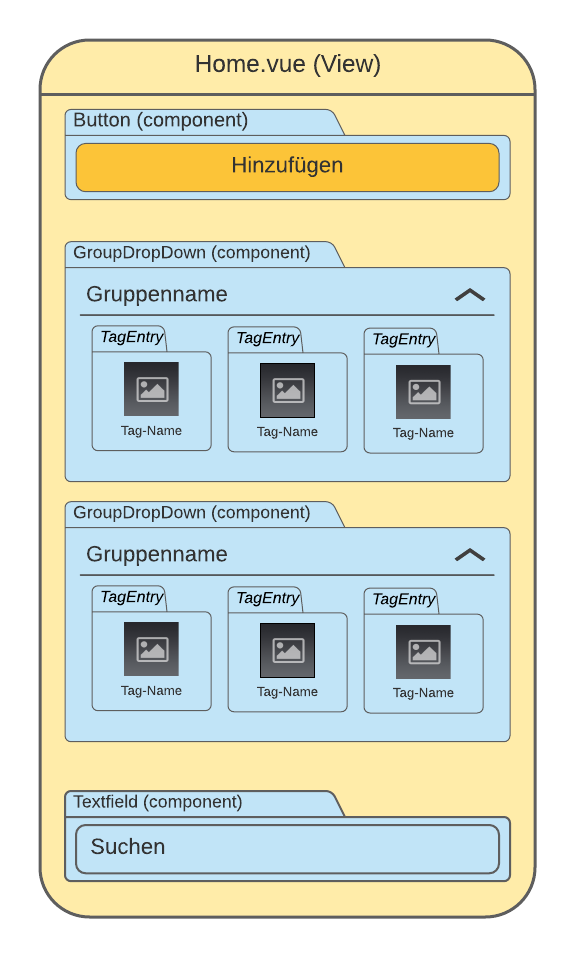
\includegraphics[width=5.9cm]{HomeScreenSchema.png}}{Schematischer Aufbau Home.vue}
Im HomeScreen sollten alle angelegten Tags gruppiert angezeigt werden. Hierfür wurden zwei \textit{components} angelegt. Die Erste (\textit{TagEntry})
enthält das Bild und den Namen eines NFC-Tags und kann in der Anwendung vielseitig wiederverwendet werden. Die Zweite \textit{component} mit dem Namen
\textit{GroupDropDown} repräsentiert eine Gruppe, zu der ein NFC-Tag gehört.
Pro NFC-Tag in der jeweiligen Gruppe wird eine Instanz der \textit{TagEntry component} in die Gruppe geladen.
Zusätzlich erhielt die \textit{GroupDropDown component} die Funktionalität auf- und
zuklappbar zu sein. \\
Diese \textit{components} werden in \textit{Home} angezeigt. Neben der Einbindung von einer \textit{GroupDropDown component} pro Gruppe
wurde im Kopfbereich noch die vom Team erstelle \textit{Button component} verwendet, die das Anlegen eines neuen NFC-Tags einleiten sollte.
Im Fußbereich befindet sich eine Suchleiste, die das Filtern der angezeigten NFC-Tags ermöglichen soll.
Die beiden letztgenannten Features waren zu diesem Zeitpunkt noch nicht umgesetzt.

\paragraph*{Entwicklung der \glqq Tag hinzufügen\grqq{} Funktionalität}
Um dem Benutzer das Hinzufügen von neuen NFC-Tags zur ermöglichen, wurde eine neue \textit{View} mit dem Namen \textit{AddTag} erstellt, welche wie auch
die \textit{Home}-View in Kopf-, Haupt- und Fußbereich eingeteilt ist. Beim Laden der View wird eine neue Instanz der Klasse \textit{NFC-Tag} erstellt.
\\~\\
\wrapfiguresafe{r}{0mm}{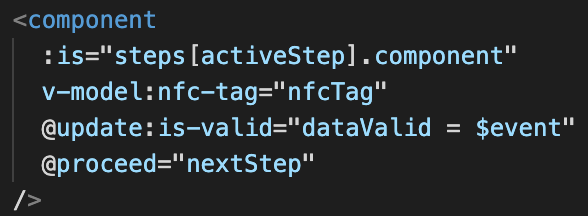
\includegraphics[width=4cm]{AddSteps.png}}{AddTag components}
Im Hauptbereich der \textit{View} werden die vier \textit{components}, die für die Eingabe der NFC-Tag Daten zuständig sind, dynamisch geladen.
Hierfür wird der beim Laden erstellte NFC-Tag (\textit{newTag}) an alle \textit{components} nacheinander weitergegeben und in ihnen mit Informationen gefüllt.
Der Fußbereich enthält abhängig von der im Hauptbereich gerade aktiven \textit{component}, \textit{Button components} für \glqq Zurück\grqq{}, \glqq Weiter\grqq{} und
\glqq Anlegen\grqq.
Alle der folgenden \textit{components} beinhalten Validierung für die eingegebenen Daten, sodass sichergestellt wird, dass das \textit{newTag} jederzeit gültige Daten besitzt.
Bei Änderung der Werte in den \textit{components} wird das Event \textit{update:is-valid} ausgelöst und in \textit{AddTag} die\textit{Disabled}-Eigenschaft des sich in der Fußzeile befindliche Button abhängig vom der Gültigkeit verändert.
So kann in jedem Schritt nur fortgefahren werden, wenn alle Eingaben die korrekte Form haben.
Alle diese \textit{components} werden ebenfalls für die Bearbeitung der NFC-Tags wiederverwendet.
\\~\\
%AddStepScan
\wrapfiguresafe{r}{0mm}{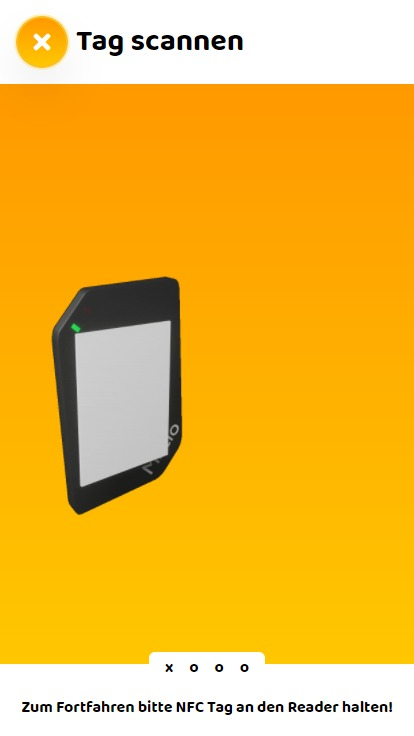
\includegraphics[width=4cm]{AddStepScan.jpeg}}{Step Scan (Add)}
Die Erste \textit{component}, welche in den Hauptbereich geladen wird, ist \textit{TagStepPlaceTagOnReader}. Dieser beinhaltet einen Text und ein \textit{GIF},
welches den Benutzer zum Scannen des NFC-Tags auffordert. Im \textit{TypeScript}-Code wird im \textit{Lifecycle Hook onMounted} an das \textit{patch}-Event des
NFC-Readers der Aufruf der Funktion \textit{attachedTagListener} gebunden. Wird nun ein NFC-Tag gescannt, führt der \textit{NFC-Reader Microservice} mittels Feathers ein Update (Aufruf des \textit{Patch}-Events) auf den \textit{NFC-Reader} durch und setzt das Attribut \textit{attachedTag} auf die gescannte NFC-ID.
Anschließend wird geprüft, ob ein NFC-Tag mit dieser ID bereits in der Datenbank vorhanden ist und der Benutzer in diesem Fall an die \textit{View} zum Bearbeiten des Tags weitergeleitet.
Ist der NFC-Tag noch nicht angelegt, wird die ID an die \textit{ID-Property} des \textit{newTag} gebunden und die Events \textit{update:nfc-tag} und \textit{proceed} ausgelöst.
\textit{update:nfc-tag} bewirkt, dass das Attribut \textit{TagId} des \textit{newTag} gesetzt wird.
\textit{proceed} weist \textit{AddTag} an, die nächste \textit{component} in den Hauptbereich der \textit{View zu laden}.
Dabei wird die Funktion \textit{attachedTagListener} vom \textit{patch}-Event abgemeldet.
\\~\\
%AddStepInfo
\wrapfiguresafe{r}{0mm}{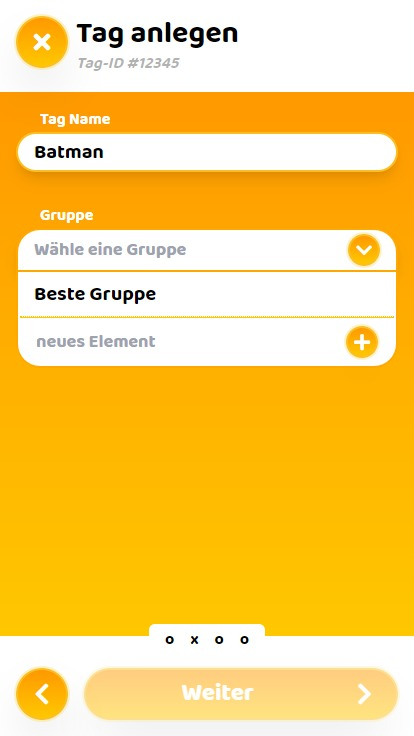
\includegraphics[width=4cm]{AddStepInfo.jpeg}}{Add Step Scan-Tag}
Als Nächstes wird die \textit{TagStepInfo component} geladen.
Sie beinhaltet eine \textit{Textbox component} für den Namen des NFC-Readers.
Diese erhält als \textit{v-model} eine \textit{computed property}\footnote{\url{https://v3.vuejs.org/guide/reactivity-computed-watchers.html}}.
Diese ruft im \textit{setter} die Methode \textit{updateTag} auf, welche die zwei Parameter \textit{key} und \textit{value} erwartet, um die Eigenschaft \textit{key} (in diesem Fall \glqq name\grqq{}) auf den im Parameter \textit{value} übergebenen Wert zu setzten.
Als Zweite \textit{component} kommt ein \textit{DropDown} zum Einsatz,
welches die Auswahl der Gruppe ermöglicht. Hierbei kann sowohl aus bereits bestehenden Gruppen gewählt, als auch direkt in der \textit{component} eine neue erstellt
werden. Auch hier wird die Methode \textit{updateTag} verwendet, die in diesem Fall mit dem Wert \glqq group \grqq{} für den Parameter \textit{key} aufgerufen wird. Der eingegebene Name und die Gruppe werden an die jeweiligen Eigenschaften von \textit{newTag} gebunden und das Event \textit{update:nfc-tag} aufgerufen, wodurch die \textit{View AddTag} den Wechsel zur nächsten \textit{compontent} einleitet.
\\~\\
%AddStepTrack
\wrapfiguresafe{r}{0mm}{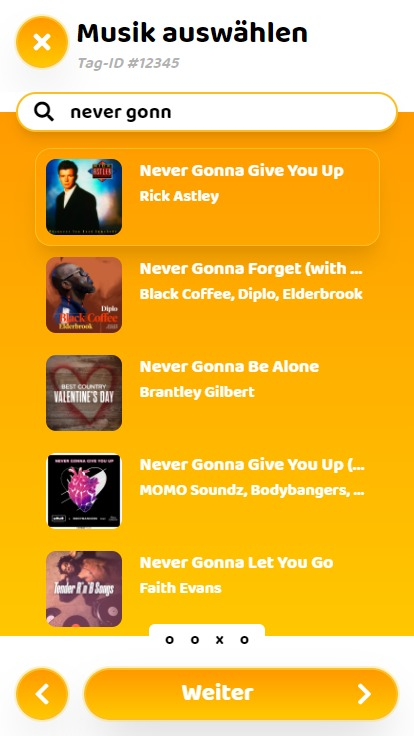
\includegraphics[width=4cm]{AddStepTrack.jpeg}}{Add Step Track}
Hier in der \textit{TagStepTrack} erhält der Benutzer die Möglichkeit, den Song auszuwählen, der beim Scannen des NFC-Tags abgespielt werden soll.
Der gewünschte Song-Titel oder Suchwörter können in eine \textit{Textbox component} eingeben werden. Zum Abrufen der Songs von Spotify wurde der \textit{SpotifyTrackService} erstellt, in dem die Methode \textit{find} überschrieben wurde.
Diese beinhaltet den Aufruf der Funktion \textit{searchTracks} der \textit{Spotify Web Api}, welcher als Parameter der in der Suchtextbox eingegebene Text übergeben wird.
Für jeden zu dem übergeben Text passenden Titel wird dann eine Instanz der erstellten Klasse \textit{Track} erstellt, die Informationen über die \textit{URL}, den Titel, die \textit{Bild-URL}, und die Künstler erhält. Das Array mit den passenden \textit{Track}-Instanzen wird anschließend an \textit{TagStepTrack} zurückgegeben und die Infos mit Bild, Titel und Interpreten angezeigt. Die Auswahl erfolgt dann per Klick auf den gewünschten Song.
Bestätigt wird die Auswahl per Klick auf \glqq Weiter\grqq{} in der Fußzeile.
Dadurch wird \textit{update:nfc-tag} Event ausgelöst und die letzte \textit{component} in die \textit{AddTagView} geladen.
\\~\\
%AddStepImage
\wrapfiguresafe{r}{0mm}{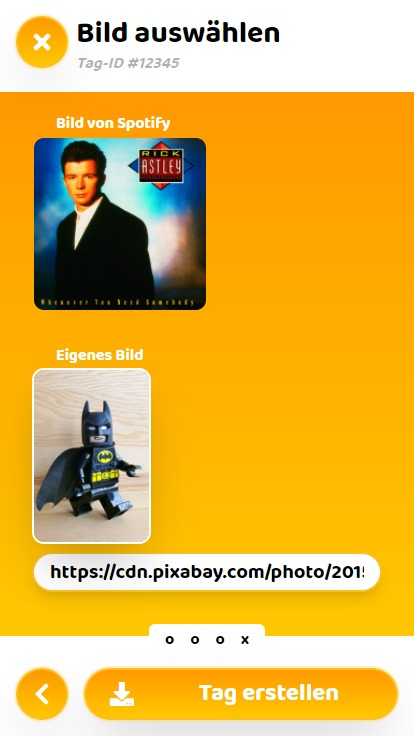
\includegraphics[width=4cm]{AddStepImage.jpeg}}{Add Step Image}
Zuletzt kann im \textit{TagStepImage} das gewünschte Bild für den NFC-Tag ausgewählt werden.
Standardmäßig wird hier das Albumcover des Songs ausgewählt, welches in \textit{AddStapTrack} bereits gesetzt wurde.
Um sicherzustellen, dass die Albumcover jederzeit aktuell sind, wird in der Datenbank nicht das Bild, sondern lediglich die URL des Bildes gespeichert.
Sollte der Musik-Streaming-Anbieter dieses ändern, wird so automatisch auch das Albumcover in der Applikation geändert.
Dies hat außerdem den Vorteil, dass die Anwendung wesentlich speicherplatzeffizienter ist, da statt teilweise sehr großen Bilddateien jeweils nur die URL gespeichert wird.
Um dem Benutzer mehr Freiheiten in der Gestaltung zu geben, kann alternativ auch ein eigenes Bild verwendet werden.
Dieses muss in der aktuellen Version auf einem Online-Dienst vorliegen.
Ist dies gewünscht, kann in einer entsprechenden Textbox die \textit{URL} dieses Bildes eingetragen werden, worauf das Bild automatisch zur Vorschau in ein dafür vorgesehenes Vorschaufeld geladen wird.
Dies stellt sicher, dass der Benutzer nicht versehentlich eine falsche Bild-URL wählt.
Zusätzlich wird diese Textbox zusätzlich mittels eines \textit{RegEx} geprüft, um sicherzustellen, dass es sich um eine nutzbare Bilddatei handelt.
Zur Bestätigung muss entweder auf das Albumcover oder auf das eigene Bild geklickt werden.
Das Erstellen des Tags kann dann mit einem Klick auf \glqq Anlegen\grqq{} im Fußbereich der \textit{View} abgeschlossen werden.
%Probleme
Durch die angestrebte Unabhängigkeit musste besonders viel Arbeit investiert werden, um die Features miteinander zu verbinden.
Dieser Prozess dauerte länger als erwartet und forderte eine hohes Maß an Kommunikation zwischen den Teammitgliedern.
Teilweise enstanden Wartezeiten und funktionierender Code wurde, über mehrere Merges, unstabil oder defekt.
Kurz vor dem Review musste noch viel getan werden, um eine reibungslose Präsentation zu garantieren.

%Lösungen
Nachdem die ersten großen Merges abgeschlossen wurde, entschied das Team eine interne und anonyme Evaluation der Teammitglieder zu starten.
Jedes Teammitglied hatte somit konstruktive Kritik aber auch Lob und Unterstützung erhalten und konnte an den eigenen Schwächen arbeiten und Stärken weiter ausbauen.
Darüber hinaus wurde auch beschlossen, in den folgenden Sprints die Menge an zu bearbeitenden Issues besser festzulegen.
%Product Increment
Das Produkt wurde um die Grundfunktionen erweitert.
Es ist nun möglich, Tags anzulegen und entsprechend den Namen, Musik und ein Bild festzulegen.
Genauso ist es dem Nutzer nun möglich, alle angelegten Tags zu durchsuchen.
Es wurde weiterhin auch das Design Mockup von dem von macio gestellten Designer in Vue größtenteils umgesetzt.
Für die Entwickler wurden auch die automatisierten Tests um einen Test auf Typsicherheit erweitert.
%Retrospektive
Besonders gut gefiel dem Team das Teamklima, vor allem des ehrliche Miteinander.
Trotz Komplikationen und Probleme konnte dem Kunden am Ende ein funktionierendes Product Increment geliefert werden.
Pull Requests und Tickets wurden besser beschrieben, sodass Probleme verständlicher waren.
Vor allem durch das interne Team Review wurde die Zusammenarbeit weiter verbessert.
Das Team konnte das Wissen zu Vue, vor allem die Themen Reaktivität, Events und Kommunikation zwischen Komponenten ausbauen.
Insgesamt war das Zeitmanagement verbesserungswürdig, da sich für einzelne Tickets zu viel Zeit genommen wurde.
Das Team stimmte überein, dass eine bessere Planung sowie Abstimmung für die nächsten Meilensteine notwendig wäre.
Auch sollte eine frühere interne Deadline gesetzt werden, damit nicht kurz vor dem Sprintende noch viele Fehler auftreten und behoben werden müssen.
Um insgesamt auch die Arbeit kontinuierlicher zu gestalten, sollten Aufgaben in kleinere Probleme aufgeteilt werden.

\subsubsection*{Meilenstein 5} $~$ \\
Mit dem fünften Meilenstein, der zwischen dem 14.01.2021 und 28.01.2021 stattfand, sollte die Entwicklung am Produkt weitgehend abgeschlossen werden, sodass der Fokus auf den Bericht gelegt werden konnte.

%Ziel
Geplant war die letzten Anwendungszenarien final umzusetzen, sodass die folgenden beiden Meilensteine zum Beheben kleinerer Fehler genutzt werden konnten.
Somit war das Ziel die Umsetzung einer \textit{View} für die Einstellungen der \textit{Leek Box}, als auch der Tags.
Außerdem sollten die User Interface Elemente, sofern noch nicht geschehen, ein einheitliches Design erhalten.
Die Dokumentation zur Bedienung der \textit{Leek Box} sollte fertiggestellt und mit der Arbeit am Bericht begonnen werden.

% Durchführung
Die \textit{View} für die Einstellungen der \textit{Leek Box} wurde hinzugefügt, die durch ein Zahnrad auf der Startseite aufgerufen werden kann.
In diesen Einstellungen können die Nutzer nun den Lautsprecher für die Wiedergabe auswählen und sehen, mit welcher Email-Adresse sie angemeldet sind. Außerdem enthält die Ansicht einen Button um sich auszuloggen.
\paragraph*{Flow-Charts} $~$ \\
\begin{wrapfigure}{r}{0cm}
  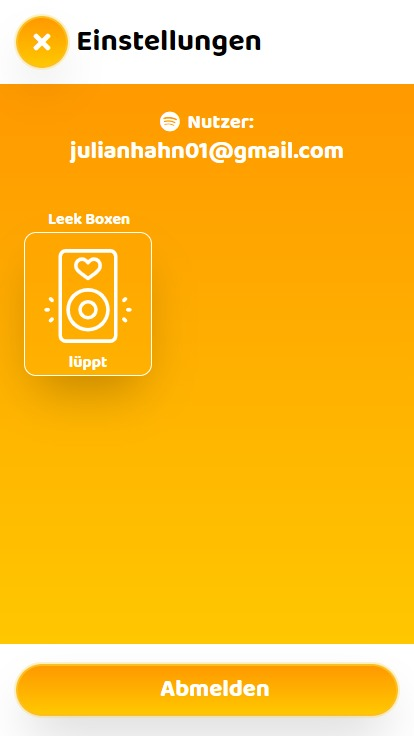
\includegraphics[width=0.45\textwidth]{Settings.jpeg}
  \caption{Leek Box Einstellungen}
\end{wrapfigure}
Auch war nun das Bearbeiten der Tags möglich.
Dabei handelte es sich lediglich um die beim Anlegen eingestellten Informationen: Name, Lied und Bild des Tags.
\paragraph*{Flow-Charts} $~$ \\
\begin{wrapfigure}{r}{0cm}
  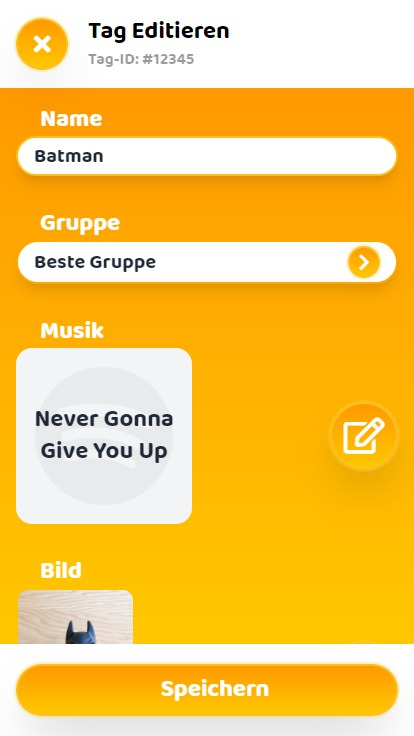
\includegraphics[width=0.45\textwidth]{TagDetails.jpeg}
  \caption{Tag Einstellungen und Details}
\end{wrapfigure}
In gekürzter Form sah der Quellcode für den Hauptinhalt des \textit{Views} wie folgt aus:
\begin{lstlisting}
<LabeledInput label="Name">
  <Textfield v-model="nfcTag.name" placeholder="z. B. Mario Figur"/>
</LabeledInput>

<LabeledInput label="Gruppe">
  <Dropdown
    v-model="nfcTagGroup"
    v-model:items="tagGroupListItems"
    :removeable="false"
    placeholder-text="Waehle eine Gruppe"
    :enable-add-item="true"
  />
</LabeledInput>

<LabeledInput label="Musik">
  <div>
    <div>
      <img
        src="/src/assets/spotify.png"
      />
      <span v-if="nfcTagTrack">{{
        cut(nfcTagTrack.title, 42)
      }}</span>
    </div>
    <Button
      icon="far fa-edit"
      text="Musik aendern"
      :to="{ name: 'tag-edit-track' }"
    />
    <Button
      icon="far fa-edit"
      :to="{ name: 'tag-edit-track' }"
    />
</LabeledInput>

<LabeledInput label="Bild">
  <div>
    <TagEntry
      v-if="nfcTag.imageUrl === 'spotify' && nfcTagTrack"
      :img="nfcTagTrack.imageUri"
    />
    <TagEntry v-else :img="nfcTag.imageUrl" />
    <Button
      icon="far fa-edit"
      :to="{ name: 'tag-edit-image' }"
    />
    <Button
      icon="far fa-edit"
      text="Bild aendern"
      :to="{ name: 'tag-edit-image' }"
    />
  </div>
</LabeledInput>
\end{lstlisting}
An dieser Stelle zeigte sich erneut die Vorzüge von Frameworks wie  \textit{Vue}, da somit die bereits vorhandenen \textit{components} wiederverwendet werden konnten.
Um ein gleiches Design der Überschriften der einzelnen Inputs zu haben, wurden hier insgesamt vier \textit{LabeledInput} genutzt, für den Namen, die Gruppe, die Musik und das Bild.
Für das ändern des Namens wurde \textit{TextInput} genutzt, dem \textit{nfcTag.name} übergeben wird.
Die Auswahl einer anderen Gruppe erfolgt über das eigene \textit{Dropdown} gelöst, der \textit{nfcTagGroup} und \textit{tagGroupListItems} übergeben bekommt.
Für die Musik wurde ein Feld mit dem derzeitigen Titel angezeigt, und daneben ein \textit{Button}, der bei einem Klick in einen anderen \textit{View} weiterleitet.
Selbiges Verfahren wurde auch für das Bild verwndet, welches angezeigt wird und daneben ein \textit{Button} auf ein anderes \textit{View} weiterleitet.

% Visualisierung des ausgewählten Tags
Um dem Nutzer zu signalisieren, ob ein Tag ausgewählt wurde, wurde in \textit{Home.vue} ein weiteres Attribut \textit{selectedTag} angelegt.
Jedem Tag-Element auf der Startseite wurde ein \textit{OnClick Listener}, welcher bei einem Klick das jeweilige Element als \textit{selectedTag} setzt hinzugefügt.
\begin{lstlisting}
const toggleTag = (tag: NFCTag): void => {
  selectedTag.value =
    tag === selectedTag.value ? null : tag;
  buttonTransitionActive.value = true;
};
\end{lstlisting}
Um dynamisch die CSS-Klasse der ausgewählten Tags zu ändern, wurde an dieser Stelle bei den \textit{TagEntrys} der ternärer Operator genutzt.
Je nachdem ob der \textit{TagEntry} der gleiche wie der \textit{selectedTag} war, wurden diesem andere Klasseneigenschaften gegeben.
\begin{lstlisting}
<TagEntry
  v-for="entry in group.tags"
  :key="entry.nfcData"
  class="m-4 w-2/6 flex-shrink-0 text-4xl"
  :class="{ 'opacity-25': selectedTag !== entry && selectedTag !== null }"
  :img="entry.imageUrl"
  :name="entry.name"
  @click="toggleTag(entry)"
/>
\end{lstlisting}
Wurde nun also ein Tag ausgewählt, wurden allen anderen die Klasse \lstinline{opacity-25} zugewiesen, was einer Tranzparenz von 25\% entsprach.

% Initial Setup
\colorbox{red}{explain this:} https://github.com/project-leek/project-leek/pull/319/files

Im Sprint wurde auch das Produkt auf Auslieferbarkeit getestet, indem das komplette Setup durchgeführt wurde.
Dabei wurde ein Setup-Guide\footnote{https://github.com/project-leek/project-leek/blob/docs/Build.md} entwickelt, sodass andere Nutzer ihre eigene \textit{leek-box} bei sich einrichten könnten.

%Probleme
Wie bereits beim vorherigen Meilenstein gestaltete sich auch hier das Zeitmanagement schwierig.
Das Team hätte in diesem Sprint mehr Tickets umsetzen und dem Kunden präsentieren können, als zu Beginn versprochen. Jedoch fehlte die Zeit um die Features genügend zu testen und entsprechend fehlerfrei dem Kunden präsentieren zu können.
Somit beschloss das Team dem Kunden im Review nur die anfänglich geplanten Featuers vorzustellen und die zusätzlichen Tickets im nächsten Sprint zu vollenden.
Das Produkt konnte um die Einstellungen der \textit{Leek Box} und die \textit{TagDetails}  erweitert werden.
Auch der Setup Guide wurde fertiggestellt, sodass ein Nutzer selbstständig eine eigene \textit{Leek Box} einrichten könnte.
Bei dem Design wurden, bis auf ein paar Kleinigkeiten die im folgenden Milstone behoben wurden, alle Unstimmigkeiten beseitigt.

%Retrospektive
Das Team erhielt vom Kunden für das bisher entstandene Produkt viel Lob.
Da das Team viel Gefallen an dem Projekt gefunden und entsprechend viel Energie aufgewendet hat, war dieses Lob sehr wertvoll und motivierend.
Das Team konnte außerdem weitere Vue Funktionen kennenlernen.
\colorbox{red}{inject provide}
Problematisch war es, dass manche Tickets von mehreren Entwicklern zeitgleich oder nacheinander bearbeitet wurden, sodass einige der getätigten Änderungen redundant waren.
Außerdem erfolgte die Kommunikation von größeren Änderung an jedes Teammitglied teilweise nur lückenhaft.
Nach der Retrospektive wurde dies dem Team deutlich und es wurde sich auf eine bessere Kommunikation geeinigt.
Lösungsvorschläge waren Verbesserung des Zeitmanagements durch \colorbox{yellow}{???} und eine bessere Kommunikation durch Festhalten von größeren Änderungen in den Pull Requests und Markierung aller Gruppenmitglieder.

\subsubsection*{Meilenstein 6} $~$ \\
Mit dem Meilenstein sechs vom 28.01.2021 bis zum 15.02.2021 sollte die Entwicklung beendet und der Fokus komplett auf den Bericht gelegt werden, sodass der nächste und letzte Meilenstein für die letzten Korrekturen im Bericht genutzt werden konnte.
%Ziel
Neben der Fokussierung auf den Bericht sollte auch das User Interface auf einheitliches Design überprüft und die Entwicklung und Fehlerbehebung abgeschlossen werden.
%Probleme
\colorbox{red}{TODO:}schlauchiger start in den report

%Lösungen
\colorbox{red}{TODO:}Welche Lösungen haben wir gefunden?

%Product Increment
Als letzte Änderungen am Produkt hat nun der Nutzer die Möglichkeit, verschiedene Leek Boxen auszuwählen bzw. neu eingerichtete Leek Boxen mit seinem Konto zu verbinden.
Die letzten Bugfixes wurden umgesetzt sowie wurden die letzten Details aus dem Design Mockup übernommen.
%Retrospektive
\colorbox{red}{TODO:}Was haben wir dabei gelernt? Neue Erkentnisse? Neue Sichtweisen?
Was lief gut, neu gelernt, was lief nicht so gut, was verbessern?

\subsubsection*{Meilenstein 7} $~$ \\
Der finale Meilenstein sieben vom 15.02.2021 bis zum 05.03.2021 sollte nur noch die letzten Korrekturen des Berichtes und Vorbereitung der Finalen Abgabe beinhalten.
\colorbox{red}{TODO:}Kurze Einleitung, von, bis
%Ziel
\colorbox{red}{TODO:}was haben wir uns vorgenommen, was war das ziel, was wollten wir schaffen?
%Probleme
\colorbox{red}{TODO:}welche prrobleme sind aufgetreten?

%Lösungen
\colorbox{red}{TODO:}Welche Lösungen haben wir gefunden?

%Product Increment
\colorbox{red}{TODO:}Was ist am Ende dabei rumgekommen?

%Retrospektive
\colorbox{red}{TODO:}Was haben wir dabei gelernt? Neue Erkentnisse? Neue Sichtweisen?
Was lief gut, neu gelernt, was lief nicht so gut, was verbessern?


\section{Fazit}
\subsection{Probleme, Lösungen, Erkenntnisse}
\colorbox{red}{TODO: Finde TITEL:} Fazit oder nur Erkenntnisse oder oder?
\colorbox{red}{Besseres Intro zum Kapitel?}
Das Projekt Informatik gab einen realistischen Einblick in die Arbeitswelt.
Das Team musste sich klassischen Alltagsproblemen stellen, Lösungswege finden und konnte wichtige Erkenntnisse für die Zukunft daraus ziehen.
Auch Coding-Entwurfsmuster und -Konventionen wurden neu erlernt und praktisch angewandt.
$~$ \\
%Einarbeitung in neue Technologien
Zu Beginn des Projektes bestand eine größere Differenz, inwieweit die einzelnen Teammitglieder mit den jeweiligen Technologien vertraut waren.
Insbesondere die Projektstruktur bereitete eine größere Einstiegshürde für viele Entwickler.
Sie wurde durch das automatische generieren von Dateien und Ordnern immer komplexer.
Mit zunehmender Entwicklungszeit und durch die Arbeit an den Teilkomponenten des Mono-Repositorys gewannen die Entwickler jedoch schnell mehr Überblick über die Struktur.
Das Team lernte wie Frameworks und Libraries  z. B. Vue, Tailwind und Feathers sinnvoll und hilfreich eingesetzt werden können.
$~$ \\
%Versionskontrolle und Deployment Cycle
Zwar wurde den Studierenden im Studium der Vorteil von Versionskontrollsystemen wie Git vermittelt, doch fand sich selten ein praktisches Anwendungszenario, dass Git über die Hauptfunktion der Versionierung hinaus sinnvoll genutzt hat.
Dieses Projekt bot erstmals eine sinnvolle Anwendung von \textit{git}.
Die Umsetzungen der gängigen Industriestandarts we z.B Pull-Requests und Code Reviews lehrte uns die Vorteile von Git in einer komplexen Umgebung.
Diese Methoden führten zu folgenden maßgebliche Verbesserungen:
Mit zwei erfordelichen Code Reviews pro Pull Request, konnten Fehler im Code häufiger entdeckt werden und so eine höhere Codequalität erreicht.
Als positiver Nebeneffekt konnten die Reviewer außerdem während des Prozesses neue Funktionen und Codemuster erlernen, zu denen sie bei Bedarf (per Kommentar) Fragen stellen konnten.
Die Gewöhnung an diesen Deployment Cycle brauchte eine gewisse Zeit, fand aber von Sprint zu Sprint immer mehr Wertschätzung im Team.
$~$ \\
%Automatisierte Tests und Deployment
Jeder Pull Request durchlief mehrere automatisierte Tests - sogenannte \textit{Actions} - die den geänderten Code auf Korrektheit in Syntax und simplen Semantischen fragen getestet haben.
Inhaltliche Funktionen der Applikation wurden durch die Tests nicht abgedeckt.
Diese prüften den Quellcode anhand fest eingestellter Testparameter.
Durch diese Tests wurde dem Team viel manuelle Arbeit abgenommen und die Fehlerquelle Mensch minimiert.
Änderungen im Master werden automatisch verarbeitet. Die neue Version des Codes wird auf Github.io veröffentlicht und geänderte Latex Dateien als PDF im eigenen Branch erstellt.
Für Pull Requests wurde ebenfalls eine Vorschau erstellt und auf einer \colorbox{yellow}{temporären} Webseite veröffentlicht.
Dank dieser Automatisierungen konnte sich das Team mehr auf das Weiterentwickeln des Projektes konzentrieren.

%Regelmäßige Standups und Retrospektiven
Durch die regelmäßigen Standups entstand ein Ort für den Austausch von Problemen und Informationen über Fortschritt und neue Funktionen.
So wurde verhindert, dass Probleme untergingen, neues Wissen wurde schneller verbreitet und die gesamte Teamproduktivität verbessert.
Das bei den Retrospektiven entstandene Feedback erwies sich als sehr wichtig für das Teamklima.
Auch die hierbei angesprochenen Probleme und Verbesserungsvorschläge wurden vom Team als sehr wertvoll für die nächsten Sprints erkannt und entsprechend adaptiert.

%Kommunikation und Eigeninitiative
Anfänglich hat sich das Team zu sehr auf die Standups, als alleiniges Kommunikationsmittel verlassen, wodurch die Absprache zwischen den Teammitgliedern nur selten statt gefunden hat.
Der Umfang erster Tickets war deutlich zu groß.
Die Komplexität eines Tickets hat Teammitglieder davon abgehalten sich mit der Thematik zu beschäftigen.
Da konkrete Fragen bei einem gänzlich neuen Thema schwierig zu formulieren sind, wurde oft komplett auf Hilfe verzichtet und das Ticket zur Seite gelegt.
Lösungsansätze wurden gemeinsam in den Retrospektiven erarbeitet.
Weiterhin konnte offen über Probleme gesprochen werden, indem teaminterne Evaluationen stattgefunden haben.

%Planung, Zielsetzung und Einschätzung
Größere Probleme hatte das Team mit dem Zeitmanagment der einzelnen Ticket.
Während eines Milestones wurden manchmal nicht alle geplanten Tickets fertiggestellt, oder es wurde nachträglich zu viel in den Sprint neu Aufgenommen.
Beides resultierte in Überstunden und zu wenig Zeit fürs Testen am Ende eines Meilensteins.
Aus diesen Erfahrungen, hat das Team gelernt wie wichtig es ist die Planung des Meilensteins und dessen Tickets besonders sorgfältig zu gestalten.
So hat das Team sich auch vorgenommen, mindestens zwei Tage vor einem Sprintende alle für den Sprint benötigten Tickets fertiggestellt zu haben.
Dadurch sollte genügend Zeit geschaffen werden, um Tickets auf Korrektheit zu testen und konfliktfrei in den Master Branch mergen zu können.
Auch wenn die Lösung dieses Problem hätte effizienter behandelt werden können, war diese Methode angesichts der knappen Projektlaufzeit die effektivste.
\subsection{Ausblick}
\newpage
\section{Anhang}
\colorbox{red}{macio Projektskizze einfügen} \label{pdf:macioprojektskizze}
\label{FigmaDesigns}
\label{FlowCharts}
\colorbox{red}{BEISPIEL, DELETE THIS} Buchreferenz \cite{Literaturbeispiel:tom} oder Seitenref \cite{google}
\printbibliography
\end{document}
